% ----------------------------------------------------------
% VERSÃO ORIGINAL
% ----------------------------------------------------------
% The Current Maintainer of this work is the abnTeX2 team, led
% by Lauro César Araujo. Further information are available on
% http://abntex2.googlecode.com/

\documentclass[
	% -- opções da classe memoir --
	12pt,				% tamanho da fonte
	openright,			% capítulos começam em pág ímpar (insere página vazia caso preciso)
	oneside,			% para impressão em verso e anverso coloque twoside
	a4paper,			% tamanho do papel.
	% -- opções da classe abntex2 --
	%chapter=TITLE,		% títulos de capítulos convertidos em letras maiúsculas
	%section=TITLE,		% títulos de seções convertidos em letras maiúsculas
	%subsection=TITLE,	% títulos de subseções convertidos em letras maiúsculas
	%subsubsection=TITLE,% títulos de subsubseções convertidos em letras maiúsculas
	% -- opções do pacote babel --
	%french,				% idioma adicional para hifenização
	%spanish,			% idioma adicional para hifenização
	english,			% idioma adicional para hifenização
	brazil				% o último idioma é o principal do documento
	]{abntex2}


% ----------------------------------------------------------
% PACOTES
% ----------------------------------------------------------
% ----------------------------------------------------------
% PACOTES BÁSICOS
% ----------------------------------------------------------
\usepackage{lmodern}            % Usa a fonte Latin Modern          
\usepackage[T1]{fontenc}        % Selecao de codigos de fonte.
\usepackage[utf8]{inputenc}     % Codificacao do documento (conversão automática dos acentos)
\usepackage{lastpage}           % Usado pela Ficha catalográfica
\usepackage{indentfirst}        % Indenta o primeiro parágrafo de cada seção.
\usepackage{color}              % Controle das cores
\usepackage{graphicx}           % Inclusão de gráficos
\usepackage{microtype}          % para melhorias de justificação
\usepackage[newfloat]{minted}   % Pygments
\usepackage{nomencl}            % Necessário para o commando makeindex
\usepackage[brazilian,hyperpageref]{backref}    % Paginas com as citações na bibl
\usepackage[alf]{abntex2cite}   % Citações padrão ABNT
\usepackage{lipsum}             
\usepackage{adjustbox}
\usepackage{amsmath,amssymb}
\usepackage{siunitx}
\usepackage{booktabs}
\usepackage{longtable}
\usepackage{tabu}
\usepackage{multirow}
\usepackage{subcaption}
%\usepackage{epigraph}
\usepackage{lscape}
\usepackage{xurl}               % Quebra links longos direito
\usepackage[ruled,vlined,portuguese,onelanguage]{algorithm2e} %for psuedo code
\usepackage{tikz}
\usetikzlibrary{arrows,automata,calc,chains,fit,matrix,positioning,quotes,shadows,shapes}
\usepackage{pgfplots}
\pgfplotsset{compat=newest,compat/show suggested version=false}

% CONFIGURAÇÕES DE PACOTES
% Configurações do pacote backref
% Usado sem a opção hyperpageref de backref
\renewcommand{\backrefpagesname}{Citado na(s) página(s):~}
% Texto padrão antes do número das páginas
\renewcommand{\backref}{}
% Define os textos da citação
\renewcommand*{\backrefalt}[4]{
    \ifcase #1 %
        Nenhuma citação no texto.%
    \or
        Citado na página #2.%
    \else
        Citado #1 vezes nas páginas #2.%
    \fi}%

% Corrige bug do anexo (https://github.com/abntex/abntex2/issues/76)
\newcommand{\refanexo}[1]{\hyperref[#1]{Anexo~\ref{#1}}}

%%%%%%%%%%%%%%%%%%%%%%%%%%%%%%%%%%%%%%%%%%%%%%%%%%%%%%%%%%%%%%%%%%%%%%%%
%% TIKZ
%%%%%%%%%%%%%%%%%%%%%%%%%%%%%%%%%%%%%%%%%%%%%%%%%%%%%%%%%%%%%%%%%%%%%%%%
% Tabelas
\tikzset{square matrix/.style={
    matrix of nodes,
    column sep=-\pgflinewidth, row sep=-\pgflinewidth,
    nodes={draw,
      minimum height=#1,
      anchor=center,
      text width=#1,
      align=center,
      inner sep=0pt
    },
  },
  square matrix/.default=2em
}

% Distância entre extremidades de dois nós
\makeatletter
\def\DistanciaExtremidades(#1,#2)#3{%
\pgfpointdiff{\pgfpointanchor{#1}{west}}{\pgfpointanchor{#2}{east}}
\pgfmathsetmacro{\myheight}{veclen(\pgf@x,\pgf@y)}
\global\expandafter\edef\csname #3\endcsname{\myheight}
}
\makeatother

% Distância entre centros de dois nós
\makeatletter
\def\DistanciaCentros(#1,#2)#3{%
\pgfpointdiff{\pgfpointanchor{#1}{center}}{\pgfpointanchor{#2}{center}}
\pgfmathsetmacro{\myheight}{veclen(\pgf@x,\pgf@y)}
\global\expandafter\edef\csname #3\endcsname{\myheight}
}
\makeatother

%%%%%%%%%%%%%%%%%%%%%%%%%%%%%%%%%%%%%%%%%%%%%%%%%%%%%%%%%%%%%%%%%%%%%%%%
%% LISTA DE CÓDIGOS
%%%%%%%%%%%%%%%%%%%%%%%%%%%%%%%%%%%%%%%%%%%%%%%%%%%%%%%%%%%%%%%%%%%%%%%%
\newenvironment{code}{\captionsetup{type=listing}}{}

\makeatletter
\let\l@listing\l@figure
\def\newfloat@listoflisting@hook{\let\figurename\listingname}
\makeatother

\SetupFloatingEnvironment{listing}{%
  fileext=lol,
  listname={Lista de códigos},
  name=Código,
  placement=p,
  within=none,
  chapterlistsgaps=on}

\setminted{% bgcolor = gray!15, 
            frame = lines,
            mathescape,
            autogobble,
            %breakanywhere,
            breaklines,
            framesep = 2mm,
            baselinestretch = 1.2,
            fontsize = \footnotesize,
            linenos
}

%%%%%%%%%%%%%%%%%%%%%%%%%%%%%%%%%%%%%%%%%%%%%%%%%%%%%%%%%%%%%%%%%%%%%%%%
%% LISTA DE ALGORITMOS
%%%%%%%%%%%%%%%%%%%%%%%%%%%%%%%%%%%%%%%%%%%%%%%%%%%%%%%%%%%%%%%%%%%%%%%%
%\let\oldlistofalgorithms\listofalgorithms
%\let\oldnumberline\numberline%
%\newcommand{\algnumberline}[1]{Algoritmo~#1 -- }
%\renewcommand{\listofalgorithms}{%
%  \let\numberline\algnumberline%
%  \oldlistofalgorithms
%  \let\numberline\oldnumberline%
%}


% ----------------------------------------------------------
% CAPA E FOLHA DE ROSTO
% ----------------------------------------------------------
% ----------------------------------------------------------
% CAPA E FOLHA DE ROSTO
% ----------------------------------------------------------
\titulo{Explorando o algoritmo de Viola-Jones na detecção e reconhecimento facial}
\autor{Julio Batista Silva}
\local{São Carlos, Brasil}
\data{2018}
\orientador{Prof.~Dr.~ Alexandre Luis Magalhães Levada}
\coorientador{}
\instituicao{%
  Universidade Federal de São Carlos -- UFSCar
  \par
  Departamento de Computação
  \par
  Engenharia de Computação}
\tipotrabalho{Trabalho de Conclusão de Curso}
% O preambulo deve conter o tipo do trabalho, o objetivo, 
% o nome da instituição e a área de concentração 
\preambulo{Trabalho de conclusão de curso.}



% ----------------------------------------------------------
% CONFIGURAÇÕES
% ----------------------------------------------------------

% Configurações de aparência do PDF final

% alterando o aspecto da cor azul
\definecolor{blue}{RGB}{41,5,195}

% informações do PDF
\makeatletter
\hypersetup{
        %pagebackref=true,
        pdftitle={\@title},
        pdfauthor={\@author},
        pdfsubject={\imprimirpreambulo},
        pdfcreator={LaTeX with abnTeX2},
        pdfkeywords={abnt}{latex}{abntex}{abntex2}{trabalho acadêmico},
        colorlinks=true,            % false: boxed links; true: colored links
        linkcolor=blue,             % color of internal links
        citecolor=blue,             % color of links to bibliography
        filecolor=magenta,              % color of file links
        urlcolor=blue,
        bookmarksdepth=4
}
\makeatother

% Espaçamentos entre linhas e parágrafos
% O tamanho do parágrafo é dado por:
\setlength{\parindent}{1.3cm}

% Controle do espaçamento entre um parágrafo e outro:
\setlength{\parskip}{0.2cm}  % tente também \onelineskip

% compila o indice
\makeindex
\makenomenclature

% ----------------------------------------------------------
% INÍCIO DOCUMENTO
% ----------------------------------------------------------
\begin{document}

% Retira espaço extra obsoleto entre as frases.
\frenchspacing

% ----------------------------------------------------------
% ELEMENTOS PRÉ-TEXTUAIS
% ----------------------------------------------------------
 \pretextual

% Capa
\imprimircapa

% Folha de rosto
% (o * indica que haverá a ficha bibliográfica)
\imprimirfolhaderosto*

% ----------------------------------------------------------
% FICHA BIBLIOGRAFICA
% ----------------------------------------------------------

% Isto é um exemplo de Ficha Catalográfica, ou ``Dados internacionais de
% catalogação-na-publicação''. Você pode utilizar este modelo como referência. 
% Porém, provavelmente a biblioteca da sua universidade lhe fornecerá um PDF
% com a ficha catalográfica definitiva após a defesa do trabalho. Quando estiver
% com o documento, salve-o como PDF no diretório do seu projeto e substitua todo
% o conteúdo de implementação deste arquivo pelo comando abaixo:
%
% \begin{fichacatalografica}
%     \includepdf{fig_ficha_catalografica.pdf}
% \end{fichacatalografica}
\begin{fichacatalografica}
	\vspace*{\fill}					% Posição vertical
	\hrule							% Linha horizontal
	\begin{center}					% Minipage Centralizado
	\begin{minipage}[c]{12.5cm}		% Largura
	
	\imprimirautor
	
	\hspace{0.5cm} \imprimirtitulo  / \imprimirautor. --
	\imprimirlocal, \imprimirdata-
	
	\hspace{0.5cm} \pageref{LastPage} p. : il. (algumas color.) ; 30 cm.\\
	
	\hspace{0.5cm} \imprimirorientadorRotulo~\imprimirorientador\\
	
	\hspace{0.5cm}
	\parbox[t]{\textwidth}{\imprimirtipotrabalho~--~\imprimirinstituicao,
	\imprimirdata.}\\
	
	\hspace{0.5cm}
		1. Detecção facial.
		2. Viola-Jones.
		I. Alexandre Luiz Magalhães Levada.
		II. Universidade Federal de São Carlos.
		III. Departamento de Computação.
		IV. Explorando o algoritmo de Viola-Jones na detecção e reconhecimento facial\\ 			
	
	\hspace{8.75cm} CDU 02:141:005.7\\
	
	\end{minipage}
	\end{center}
	\hrule
\end{fichacatalografica}

%% ----------------------------------------------------------
% INSERIR ERRATA
% ----------------------------------------------------------
\begin{errata}
Elemento opcional da \citeonline[4.2.1.2]{NBR14724:2011}. Exemplo:

\vspace{\onelineskip}

FERRIGNO, C. R. A. \textbf{Tratamento de neoplasias ósseas apendiculares com
reimplantação de enxerto ósseo autólogo autoclavado associado ao plasma
rico em plaquetas}: estudo crítico na cirurgia de preservação de membro em
cães. 2011. 128 f. Tese (Livre-Docência) - Faculdade de Medicina Veterinária e
Zootecnia, Universidade de São Paulo, São Paulo, 2011.

\begin{table}[htb]
\center
\footnotesize
\begin{tabular}{|p{1.4cm}|p{1cm}|p{3cm}|p{3cm}|}
  \hline
   \textbf{Folha} & \textbf{Linha}  & \textbf{Onde se lê}  & \textbf{Leia-se}  \\
    \hline
    1 & 10 & auto-conclavo & autoconclavo\\
   \hline
\end{tabular}
\end{table}

\end{errata}


% ----------------------------------------------------------
% INSERIR FOLHA DE APROVAÇÃO
% ----------------------------------------------------------
% Isto é um exemplo de Folha de aprovação, elemento obrigatório da NBR
% 14724/2011 (seção 4.2.1.3). Você pode utilizar este modelo até a aprovação
% do trabalho. Após isso, substitua todo o conteúdo deste arquivo por uma
% imagem da página assinada pela banca com o comando abaixo:
%
% \includepdf{folhadeaprovacao_final.pdf}
%
\begin{folhadeaprovacao}

  \begin{center}
    {\ABNTEXchapterfont\large\imprimirautor}

    \vspace*{\fill}\vspace*{\fill}
    \begin{center}
      \ABNTEXchapterfont\bfseries\Large\imprimirtitulo
    \end{center}
    \vspace*{\fill}
    
    \hspace{.45\textwidth}
    \begin{minipage}{.5\textwidth}
        \imprimirpreambulo
    \end{minipage}%
    \vspace*{\fill}
   \end{center}
        
   Trabalho aprovado. \imprimirlocal, 12 de julho de 2018:

   \assinatura{\textbf{\imprimirorientador} \\ Orientador} 
   \assinatura{\textbf{Prof.~Dr.~Fredy João Valente} \\ Membro da banca}
   \assinatura{\textbf{Prof\textsuperscript{a}.~Dr\textsuperscript{a}.~Marcela Xavier Ribeiro} \\ Membro da banca}
   %\assinatura{\textbf{Professor} \\ Convidado 3}
      
   \begin{center}
    \vspace*{0.5cm}
    {\large\imprimirlocal}
    \par
    {\large\imprimirdata}
    \vspace*{1cm}
  \end{center}
  
\end{folhadeaprovacao}


\begin{dedicatoria}

    Dedico este trabalho aos meus pais, Cesar de Souza e Silva e Fátima Aparecida Batista Silva, por todo o amor, incentivo aos estudos e investimento, que foram fundamentais para a realização deste trabalho.

\end{dedicatoria}

% ----------------------------------------------------------
% AGRADECIMENTOS
% ----------------------------------------------------------
\begin{agradecimentos}
    Agradeço aos meus pais, Cesar e Fátima, que sempre me apoiaram e me ajudaram durante a graduação.
    
    À minha companheira, Louise Lobão, pelo amor e carinho, que me deram força para superar as dificuldades da vida.
    
    Ao meu orientador, Alexandre Levada, pelo apoio, atenção, paciência e conselhos.
    
    À Universidade Federal de São Carlos por oferecer recursos e acesso a grandes professores, que foram fundamentais para a minha formação.
    
    Aos meus veteranos, calouros e colegas de curso que, de alguma forma, contribuíram para a minha graduação.
    
    Aos amigos que fiz durante o intercâmbio na Alemanha.
    
    À CAPES pela bolsa que me sustentou durante o intercâmbio.
    
    Ao meu gestor, Felipe Silva, por ter sugerido o tema deste trabalho e me ajudado a equilibrar meu tempo entre trabalho e estudo.
    
    A todos da Visagio.
    
    Ao pessoal do Dragões de Garagem.

    Aos criadores do abn\TeX\ por deixar este trabalho tão bonito e bem formatado.

    Aos meus gatos, Amélia e Joaquim, que me fizeram companhia durante a escrita desta monografia.

\end{agradecimentos}


% ----------------------------------------------------------
% EPÍGRAFE
% ----------------------------------------------------------
\begin{epigrafe}
    \vspace*{\fill}
	\begin{flushright}
		\textit{``Miau, \\
		Miau, \\
		Miau. \\
		(Joaquim e Amélia, 2018)}
	\end{flushright}
\end{epigrafe}


% ----------------------------------------------------------
% RESUMOS
% ----------------------------------------------------------

% resumo em português
\setlength{\absparsep}{18pt} % ajusta o espaçamento dos parágrafos do resumo
\begin{resumo}
As inúmeras aplicações das técnicas para detecção e reconhecimento facial têm chamado muita atenção de empresas e governos. Esse crescente interesse pelo assunto atraiu investimentos em pesquisas e resultou em progressos significantes no desenvolvimento de novos métodos, bibliotecas, produtos e serviços.

Apesar de muitas dessas ferramentas serem descritas como simples e utilizáveis sem a necessidade de conhecimentos prévios em visão computacional, um embasamento teórico permite escolher as tecnologias apropriadas e usá-las de forma otimizada, considerando suas capacidades e limitações.

Este trabalho introduz as áreas de detecção e reconhecimento facial através de uma extensa revisão bibliográfica, que fornece uma visão geral sobre inúmeros métodos encontrados na literatura e apresenta uma coletânea de recursos úteis ao treinamento de classificadores e validação dos algoritmos.

Também é feito um estudo mais aprofundado sobre Viola-Jones e Eigenfaces ao apresentar o projeto e a implementação de um sistema capaz de detectar e reconhecer faces construído através da combinação desses métodos. É mostrado que a taxa de detecção do Eigenfaces não é suficiente para o uso desejado e são propostas alternativas.

O primeiro módulo desse sistema é executado em um Raspberry Pi e é um exemplo de como aliar conhecimento teórico, bibliotecas open source, ferramentas comerciais e hardware para a criação de um produto lucrativo.

 \textbf{Palavras-chaves}: Detecção facial. Viola-Jones. Reconhecimento facial. Eigenfaces. Raspberry Pi.
\end{resumo}

% resumo em inglês
\begin{resumo}[Abstract]
 \begin{otherlanguage*}{english}

The numerous applications of facial detection and recognition techniques have attracted much attention from companies and governments. This growing interest in the subject attracted investment in research and resulted in significant advances in the development of new methods, libraries, products and services.

Although many of these tools are described as simple and usable without the need for prior knowledge in computer vision, a theoretical basis allows one to choose the appropriate technologies and use them optimally, considering their capabilities and limitations.

This work introduces the areas of facial detection and recognition through an extensive bibliographic review, which provides an overview of the numerous methods found in the literature and presents a collection of useful resources for the training of classifiers and validation of algorithms.

Further study is also made on Viola-Jones and Eigenfaces while presenting the design and implementation of a system capable of detecting and recognizing faces constructed by combining these methods. It is shown that the detection rate of the Eigenfaces is not sufficient for the desired use and alternative solutions are proposed.

The first module of this system runs on a Raspberry Pi and is an example of how to combine theoretical knowledge, open source libraries, comercial tools and hardware in the creation of a profitable product.
   \vspace{\onelineskip}
 
   \noindent 
   \textbf{Key-words}: Facial detection. Viola-Jones. Facial recognition. Eigenfaces. Raspberry Pi.
 \end{otherlanguage*}
\end{resumo}

% resumo em francês 
%\begin{resumo}[Résumé]
% \begin{otherlanguage*}{french}
%    Il s'agit d'un résumé en français.
 
%   \textbf{Mots-clés}: latex. abntex. publication de textes.
% \end{otherlanguage*}
%\end{resumo}

% resumo em espanhol
%\begin{resumo}[Resumen]
% \begin{otherlanguage*}{spanish}
%   Este es el resumen en español.
  
%   \textbf{Palabras clave}: latex. abntex. publicación de textos.
% \end{otherlanguage*}
%\end{resumo}




% ----------------------------------------------------------
% inserir lista de ilustrações
% ----------------------------------------------------------
\pdfbookmark[0]{\listfigurename}{lof}
\listoffigures*
\cleardoublepage

% ---
% inserir lista de Códigos
% ---
\pdfbookmark[0]{\listlistingname}{lol}
\begin{KeepFromToc}
	\listoflistings
\end{KeepFromToc}
\cleardoublepage

% ---
% inserir lista de Algoritmos
% ---
\makeatletter
\let\l@algocf\l@figure
\makeatother
\let\oldfigurename\figurename
\renewcommand{\figurename}{\algorithmcfname}

\pdfbookmark[0]{\listalgorithmcfname}{loa}
\begin{KeepFromToc}
    \listofalgorithms
\end{KeepFromToc}
\cleardoublepage

\renewcommand{\figurename}{\oldfigurename}

% ----------------------------------------------------------
% inserir lista de tabelas
% ----------------------------------------------------------
\pdfbookmark[0]{\listtablename}{lot}
\listoftables*
\cleardoublepage

% ----------------------------------------------------------
% inserir lista siglas e abreviaturas
% ----------------------------------------------------------
% ----------------------------------------------------------
% INSERIR LISTA DE ABREVIATURAS E SIGLAS
% ----------------------------------------------------------
\begin{siglas}
  \item[FERET] Face Recognition Technology
  \item[RAM] Random Access Memory
\end{siglas}



% ----------------------------------------------------------
% inserir lista símbolos
% ----------------------------------------------------------
% INSERIR LISTA DE SÍMBOLOS
% ----------------------------------------------------------
\begin{simbolos}
  \item[$ \Gamma $] Letra grega Gama
  \item[$ \Lambda $] Lambda
  \item[$ \zeta $] Letra grega minúscula zeta
  \item[$ \in $] Pertence
\end{simbolos}


% ----------------------------------------------------------

% ----------------------------------------------------------
% inserir o sumario
% ----------------------------------------------------------
\pdfbookmark[0]{\contentsname}{toc}
\tableofcontents*
\cleardoublepage

% ----------------------------------------------------------
% ELEMENTOS TEXTUAIS
% ----------------------------------------------------------
\textual

% ----------------------------------------------------------
% Introdução (exemplo de capítulo sem numeração, mas presente no Sumário)
% ----------------------------------------------------------
% ----------------------------------------------------------
% Introdução (exemplo de capítulo sem numeração, mas presente no Sumário)
% ----------------------------------------------------------
% \chapter*[Introdução]{Introdução}
% \addcontentsline{toc}{chapter}{Introdução}
% ----------------------------------------------------------

%\chapter{Introdução}

A capacidade de identificar faces e suas emoções é um importante mecanismo neurológico para interações sociais que, em certo grau, está presente até mesmo em recém nascidos \cite{morton1991conspec} \cite{fantz1961origin}.

Enquanto humanos possuem uma notável capacidade de reconhecer faces, o desenvolvimento de sistemas computacionais com capacidade similar é uma área de pesquisa em andamento há mais de cinco décadas \cite{bledsoe1964facial} \cite{chan1965man} \cite{bledsoe1966man} \cite{bledsoe1966model} \cite{boyer1991biographical} \cite{kelly1970visual} \cite{kanade1973picture}.

O desenvolvimento de modelos computacionais para reconhecimento facial são de interesse para diversas aplicações práticas como identificação criminal, sistemas de segurança, biometria, processamento de imagens e interação humano-computador.

Infelizmente, o desenvolvimento de um sistema computacional para reconhecimento facial automatizado é bastante difícil por diversos motivos. Faces são complexas, multidimensionais e expressivas \cite{turk1991eigenfaces} e as imagens podem sofrer variações em escala, localização, ponto de visão, iluminação e obstrução \cite{censtudy}.

\section{Motivação}\label{sec:motivacao}

O desenvolvimento de novos algoritmos de processamento de imagens acompanhado do maior acesso a câmeras digitais, hardwares com alto poder de processamento, bibliotecas para visão computacional, como a OpenCV, e APIs de análise de imagem, como o Google Vision, o Microsoft Cognitive Services, o Amazon Rekognition e o IBM Watson Visual Recognition, tornou viável a implantação de sistemas com detecção e reconhecimento facial em diversas empresas e produtos.

Nos últimos anos, lojas de varejo têm usado com sucesso as tecnologias de detecção e reconhecimento facial para segurança, personalização de serviço, marketing e análise de sentimento \cite{fortune2015walmart} \cite{exame2018pontofrio} \cite{2017recfacial}.

Este trabalho explora um algoritmo de grande impacto na última década, o algoritmo Viola-Jones, e foi motivado pela implementação de um sistema de reconhecimento facial em uma rede de lojas de varejo na cidade do Rio de Janeiro.

\section{Objetivos}\label{sec:objetivos}

O objetivo deste trabalho é fornecer uma base teórica para uma futura implantação de um sistema de reconhecimento facial, através do estudo do algoritmo de Viola-Jones.


% ----------------------------------------------------------
% PARTE
% ----------------------------------------------------------
\part{Detecção Facial}

% ----------------------------------------------------------
% Capitulo com exemplos de comandos inseridos de arquivo externo
% ----------------------------------------------------------
\chapter{Detecção facial}\label{cap:detecao_facial}

\chapterprecis{Isto é uma sinopse de capítulo.}\index{sinopse de capítulo}

O papel de um detector de faces é, dada uma imagem arbitrária, determinar se ela contém faces humanas ou não e, caso positivo, retornar a localização e dimensões de cada face \cite{censtudy}.

A detecção de faces é utilizada em câmeras fotográficas para ajuste automático de foco, em softwares de imagens e redes sociais para marcação de pessoas e é uma etapa importante para o processo de reconhecimento facial. Antes de executar um algoritmo de reconhecimento facial, é de praxe realizar uma detecção facial a fim de concentrar os esforços do reconhecedor facial apenas nas áreas relevantes.

É preciso minimizar tanto a quantidade de faces não identificadas (falso-negativos) quanto objetos reconhecidos erroneamente como faces (falso-positivos) para obter uma performance aceitável. Para tanto, algoritmos de aprendizado de máquina podem ser muito úteis.

Diversas dificuldades influenciam na eficiência dos algoritmos, como ruídos, variação de iluminação, expressões faciais, imagem de fundo, orientação da cabeça, obstrução da face ou sobreposição de faces \cite{de2015processo} e, nota-se que, para análise de streamings de vídeo, é fundamental que a detecção facial seja realizada em tempo real.

Segundo, \citeonline{de2015processo}, "as técnicas mais citadas para realizar a detecção de faces são: casamento de padrões que consiste na detecção por meio de comparações com formas ométricas, modelos estatísticos, modelos baseado em redes neurais, modelos baseados em tons de pele e o Viola; Jones". Dentre os trabalhos anteriores a Viola-Jones, destacam-se \citeonline{rowley1998neural} e \citeonline{schneiderman2000statistical}.


% ----------------------------------------------------------
% Capitulo 2
% ----------------------------------------------------------
\chapter{Dicas úteis}\label{cap_dicas}

O presente capítulo foi escrito foi Roney (https://github.com/roneyfraga), que não faz parte da equipe da Equipe \abnTeX . Apenas algumas dicas serão acrescentadas.

\section{Aprender \LaTeX }
Se você não sabe por onde começar a estudar para aprender \LaTeX, segue lista de materiais que eu utilizei e que sempre recorro quando preciso:

\begin{itemize}
    \item \href{http://www.mat.ufmg.br/~regi/topicos/intlat.pdf}{Introdução ao \LaTeX} do Professor Reginaldo J. Santos.
    \item \href{http://zelmanov.ptep-online.com/ctan/lshort_port.pdf}{Uma introdução não tão pequena de \LaTeX} por Tobias Oetiker Hubert Partl, Irene Hyna e Elisabeth Schlegl. Tradução de Alberto Simões.
    \item \href{http://www.uel.br/projetos/matessencial/superior/pdfs/latexmat.pdf}{\LaTeX\ para matemática com o TeXnicCenter} de Ulysses Sodré.
    \item \href{http://en.wikibooks.org/wiki/LaTeX}{\LaTeX\ Wikibooks.}
\end{itemize}

\section{\LaTeX + R}

\begin{itemize}
    \item knitr
    \item tikz
    \item tables
    \item xtable
\end{itemize}

\section{\LaTeX + Referências}

\begin{itemize}
    \item zotero
    \item mendley
    \item google
    \item sites de revistas
\end{itemize}

\section{\LaTeX + diversos}


% ----------------------------------------------------------

% ----------------------------------------------------------
% Capitulo 3
% ----------------------------------------------------------
\chapter{Detecção facial com OpenCV}\label{cap:opencv}

%\chapterprecis{Detecção facial utilizando a biblioteca OpenCV.}

OpenCV (Open Source Computer Vision Library) é uma biblioteca multiplataforma de código aberto (licença BSD) voltada principalmente para aplicações de visão computacional em tempo real \cite{kaehler2016learning}. Ela foi lançada oficialmente em 1999 pela Intel Corporation e continua em constante desenvolvimento. \index{OpenCV}
Apesar de ser escrita em C e C++, existem interfaces em diversas outras linguagens, como Python, Java e MATLAB.

\section{Bases de faces para treino e testes}\label{sec:base_faces}
\index{Bases de faces}

Existe uma grande quantidade de bases de imagens de faces disponíveis para treinar e testar algoritmos de detecção e reconhecimento facial, cada uma com características próprias \cite{grgic2013face, huang2007labeled, mozaffari2011twins}. A \autoref{tab:bases_faces} lista alguns deles.

\begin{longtabu} to \textwidth { >{\footnotesize}X[3,l] >{\footnotesize}X[1,l] >{\footnotesize}X[1,l] >{\footnotesize}X[3,l] }
\caption{Bases de imagens de faces}
\label{tab:bases_faces}\\
\textbf{Bases de imagens}                                                            & \textbf{Indivíduos}  & \textbf{Imagens}                & \textbf{Comentários}                                                    \\\hline
\endfirsthead
\textbf{Bases de imagens}                                                            & \textbf{Indivíduos}  & \textbf{Imagens}                & \textbf{Comentários}                                                    \\\hline
\endhead
AR Face Database                                  \cite{martinez1998ar}              & 126                  & 4000                            & Pose frontal, expressão, iluminação, oclusão (óculos, cachecol)         \\\hline
AT\&T Database                                    \cite{samaria1994parameterisation} & 40                   & 400                             & Variação temporal, iluminação, expressão, óculos                        \\\hline
BANCA database                                    \cite{bailly2003banca}             & 208                  & 2496                            & Voz e face, voltado para sistemas multimodais de verificação            \\\hline
BioID Face Database                               \cite{jesorsky2001robust}          & 23                   & 1521                            & Tons de cinza, plano de fundo, iluminação, expressão, posição dos olhos \\\hline
Caltech Faces                                     \cite{weber1995caltech}            & 27                   & 450                             & Iluminação, expressão, plano de fundo                                   \\\hline
Caltech 10000 Web Faces                           \cite{angelova2005pruning}         & $\approx$ 10000      & 10000                           & Grande variedade, características faciais anotadas                      \\\hline
CAS-PEAL Face Database                            \cite{gao2008cas}                  & 1040                 & 99594                           & Expressão, acessórios, iluminação, poses múltiplas, chinês              \\\hline
CelebA                                            \cite{liu2015faceattributes}       & 10177                & 202599                          & Grande variedade, características faciais anotadas                      \\\hline
Cohn-Kanade AU-Coded Facial Expression Database   \cite{cohn1999automated}           & 100                  & 500 sequências                  & Sequência dinâmica de expressões faciais                                \\\hline
Disguise Face Database                            \cite{singh2009face}               & ?                    & ?                               & 10 variações por indivíduo usando disfarces sintéticos (barba, etc)     \\\hline
EQUINOX HID Face Database                         \cite{socolinsky2001illumination}  & 91                   & ?                               & Imagens infra vermelho, frontal                                         \\\hline
Face Video Database da Sociedade Max Planck       \cite{kleiner2004mpi}              & ?                    & 246 sequências de vídeo         & 6 pontos de vista simultâneos, vídeo                                    \\\hline
Face Recognition Grand Challenge Databases        \cite{phillips2005overview}        & > 466                & > 50000 imagens e varreduras 3D & Bem grande, iluminação, expressão, plano de fundo, 3D, sequencias       \\\hline
FEI Face Database                                 \cite{junior2006captura}           & 200                  & 2800                            & Cor, fundo branco, expressão, rotação de cabeça                         \\\hline
FERET Database (Color)                            \cite{phillips1998feret}           & 1199                 & 14126                           & Variação temporal, cor, expressão, pose e iluminação controladas        \\\hline
Georgia Tech Face Database                        \cite{georgiatechfacedatabase}     & 50                   & 750                             & Expressão, iluminação, escala, orientação                               \\\hline
Indian Face Database                              \cite{vidit2002indian}             & 40                   & > 440                           & Frontal, Índia                                                          \\\hline
Japanese Female Facial Expression                 \cite{lyons1998coding}             & 10                   & 213                             & Emoções, indivíduos femininos, Japão                                    \\\hline
Labeled Faces in the Wild                         \cite{huang2007labeled}            & 5749                 & 13233                           & Pose, iluminação, expressão, plano de fundo, diversidade                \\\hline
MIT-CBCL Face Recognition Database                \cite{weyrauch2004component}       & 10                   & > 2000                          & Imagens de modelos 3D, iluminação, pose, fundo                          \\\hline
M2VTS Multimodel Face Database (Release 1.00)     \cite{sanchez1997statistical}      & 37                   & 185                             & Grandes mudanças de pose, indivíduos falando, óculos, mudanças no tempo \\\hline
M2VTS, Extended, Univ. of Surrey, UK              \cite{messer1999xm2vtsdb}          & 295                  & 1180 vídeos                     & Rotação de cabeça, indivíduos falando, modelos 3D, alta definição       \\\hline
NIST Mugshot ID                                   \cite{watson1994nist}              & 1573                 & 3248                            & Imagens frontais e de perfil                                            \\\hline
PIE Database, CMU                                 \cite{sim2002cmu}                  & 68                   & 41368                           & Bem grande, pose, iluminação, expressão                                 \\\hline
Plastic Surgery Database                          \cite{singh2010plastic}            & 900                  & 1800                            & Imagens antes e depois de diferentes tipos de cirurgia plástica         \\\hline
Psychological Image Collection at Stirling (PICS) \cite{hancock2004psychological}    & ?                    & ?                               & Voltado para experimentos de psicologia                                 \\\hline
Synthetic Face Disguise Database                  \cite{singh2009face}               & 100                  & 4000                            & Faces sintéticas com disfarces variados                                 \\\hline
UCD Colour Face Image Database for Face Detection \cite{sharma2003colour}            & $\approx$ 299        & 299                             & Voltado para detecção, bastante variado, cor                            \\\hline
UMIST Face Database                               \cite{graham1998characterising}    & 20                   & 564                             & Pose, gênero, raça, tons de cinza                                       \\\hline
University of Essex, UK                           \cite{spacek1996university}        & 395                  & 7900                            & Diversidade racial, óculos, barbas, universitários                      \\\hline
University of Oulu Physics-Based Face Database    \cite{marszalec2000physics}        & 125                  & > 2000                          & Iluminação bastante variada, óculos                                     \\\hline
VALID Database                                    \cite{fox2005realistic}            & 106                  & 530                             & Condições de escritório altamente variáveis                             \\\hline
VidTIMIT Database                                 \cite{sanderson2008biometric}      & 43                   & Múltiplos vídeos por pessoa     & Vídeo, áudio, rotação de cabeça                                         \\\hline
Yale Face Database                                \cite{belhumeur1997eigenfaces}     & 15                   & 165                             & Tons de cinza, expressões, óculos, iluminação                           \\\hline
Yale Face Database B                              \cite{georghiades2001few}          & 10                   & 5760                            & Pose, iluminação                                                        \\\hline
Yale Face Database B Extended                     \cite{kclee05}                     & 38                   & 2452\footnotemark               & Nove poses e 64 condições de iluminação
\end{longtabu}

\footnotetext{O site diz 16128 imagens de 28 indivíduos, porém o arquivo disponível para download contém mais imagens.}


Este trabalho utilizou quatro dessas bases para treinar e avaliar o detector facial:

\begin{description}
\item [FERET] \index{Bases de faces!FERET}
É uma base de faces criada por P. Jonathon Phillips e Harry Wechsler entre 1993 e 1996 como parte do programa FERET (Facial Recognition Technology), patrocinado pelo Departamento de Defesa dos Estados Unidos.
A cópia utilizada neste trabalho foi obtida através de solicitação por email ao NIST (\textit{National Institute of Standards and Technology}).
Esta base contém 14126 imagens tiradas em condições controladas com algumas variações de ângulo e expressão.
Alguns dos indivíduos foram fotografados múltiplas vezes em diferentes anos, o que permite estudar mudanças de aparência.
Para o treino do classificador, foram selecionadas apenas 2409 fotos frontais.

\item [FEI] \index{Bases de faces!FEI}
É uma base de faces criada pelo laboratório de processamento de imagens do Centro Universitário FEI em São Bernardo do Campo. Ela é composta por 14 imagens de 200 indivíduos (100 homens e 100 mulheres), totalizando 2800 fotografias. Todas as imagens são coloridas e com fundo branco.
Para o treino do classificador, foram utilizadas 400 fotos frontais.

\item [Caltech 10000 Web Faces] \index{Bases de faces!Caltech}
É uma base que contém 10524 faces em 7092 imagens obtidas da internet. As coordenadas dos olhos, nariz e centro da boca estão anotadas em um arquivo, o que permitiu cortar as imagens para serem usadas no treinamento do classificador. Algumas imagens foram excluídas por não mostrar suficientemente o rosto, estarem muito rotacionadas ou não possuírem resolução suficiente.

\item [LFW] \index{Bases de faces!LFW}
(Labeled Faces in the Wild). É uma base de 13233 imagens coletadas da internet criado e distribuído pela universidade de Massachussetts para estudar reconhecimento facial irrestrito.
Essa base foi utilizada apenas para testar o classificador.
\end{description}


\section{Treino do Classificador}\label{sec:treino_classificador}
\index{Classificador!Treinamento}

\subsection{Imagens de treinamento}\label{sec:imagens_de_treino}

Para treinar um classificador, é preciso um conjunto de imagens positivas (imagens contendo faces) e um conjunto de imagens negativas (imagens de fundo).

\citeonline{viola2004robust} usaram 4916 imagens positivas e 9500 imagens negativas, posteriormente, \citeonline{lienhart2003empirical} concluíram que, nas condições usadas por eles, utilizar mais do que 5000 imagens positivas e 3000 imagens negativas traz pouco benefício para o resultado do treinamento.

Imagens positivas podem ser obtidas de alguma base listada na \autoref{sec:base_faces}. Se a base escolhida não possuir uma quantidade suficiente de exemplos, é possível aplicar transformações como rotação, inversão e alteração de intensidade às imagens existentes.

Após obter imagens positivas, é preciso identificar onde as faces estão localizadas utilizando um arquivo com formato específico, no qual cada linha contém o caminho da imagem, a quantidade de faces marcadas e coordenadas que descrevem retângulos em volta das faces.

O OpenCV possui uma ferramenta chamada \texttt{opencv\_annotation} que permite marcar com o cursor do mouse as regiões contendo faces. O comando para executá-la é \mintinline[breaklines]{bash}{opencv_annotation --annotations=/diretorio/anotacao.txt --images=/diretorio/das/imagens/}, como mostra a \autoref{fig:opencv_annotation}. 

\begin{figure}[htbp]
   \caption{Ferramenta de anotação do OpenCV}
   \label{fig:opencv_annotation}
   \begin{center}
     \scalebox{0.6}{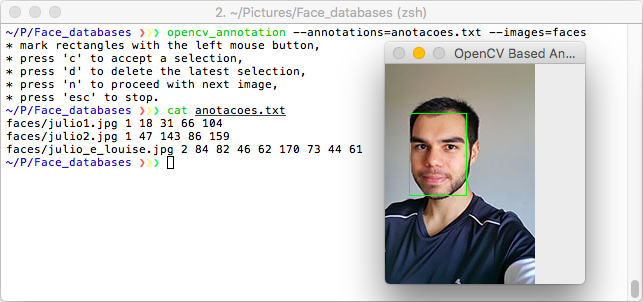
\includegraphics{imagens/opencv_annotation.png}}
   \end{center}
\end{figure}

Se as imagens contiverem apenas faces já cortadas, é possível gerar o arquivo de anotações com o comando \mintinline[breaklines]{bash}{find positivas/ -name "*.jpg" -exec identify -format '%i 1 0 0 %w %h\n' {} \; > anotacoes.txt}.

Também é preciso listar as imagens negativas, o que pode ser feito com o comando \mintinline[breaklines]{bash}{find negativas/ -name "*.jpg" > negativas.txt}.


\subsection{Treinamento}\label{sec:treinamento}

\begin{figure}[htbp]
   \caption{Criação do vetor}
   \label{fig:opencv_createsamples}
   \begin{center}
     \scalebox{0.6}{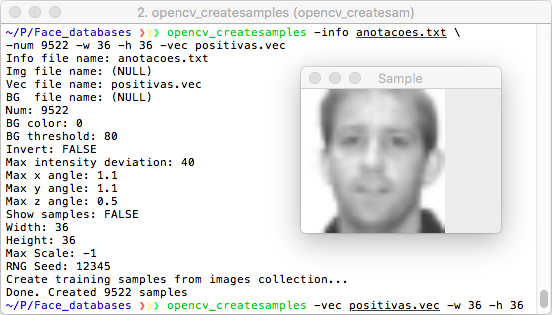
\includegraphics{imagens/opencv_createsamples.png}}
   \end{center}
\end{figure}

A OpenCV também possui ferramentas para o treinamento do classificador. 
Primeiro é necessário criar um arquivo de vetor com o comando \texttt{opencv\_createsamples}, passando a quantidade de exemplos, a largura e a altura como parâmetros. Exemplo: \mintinline[breaklines]{bash}{opencv_createsamples -info anotacoes.txt -num 2400 -w 24 -h 24 -vec positivas_24x24.vec}.

Para visualizar as imagens inseridas no vetor, basta usar o mesmo comando, mas passando o vetor como parâmetro: \mintinline[breaklines]{bash}{opencv_createsamples -vec positivas_24x24.vec -w 24 -h 24}.

Finalmente, o classificador em cascata é treinado com o comando \texttt{opencv\_traincascade}, que recebe como parâmetros um diretório onde o classificador será salvo, o arquivo de vetor gerado anteriormente, a lista de imagens negativas, a quantidade de imagens positivas e negativas, o número e estágios da cascata e as dimensões das imagens no vetor.
Exemplo: \mintinline[breaklines]{bash}{opencv_traincascade -data classificador/ -vec positivas_24x24.vec -bg negativas.txt -numPos 2000 -numNeg 1000 -numStages 10 -w 24 -h 24}.

\begin{figure}[htbp]
    \centering
    \caption{Treinamento do classificador em cascata usando \texttt{opencv\_traincascade}}
   \label{fig:opencv_traincascade}
    \begin{subfigure}[t]{0.49\textwidth}
    \centering
    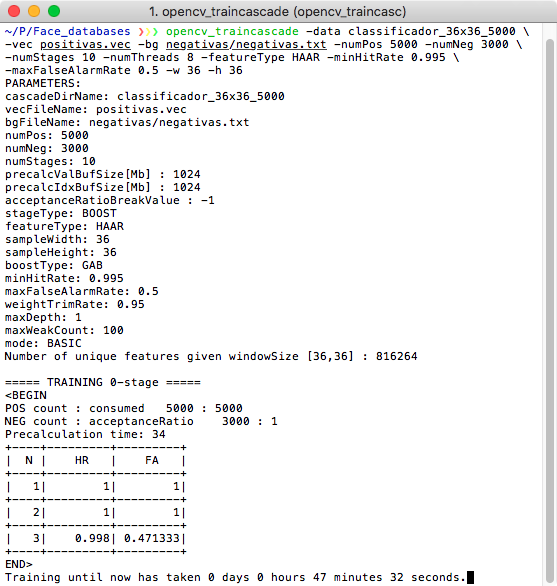
\includegraphics[width=0.95\linewidth]{imagens/opencv_traincascade_inicio.png}
    \caption{Início}\label{fig:opencv_traincascade:a}
    \end{subfigure}
    \begin{subfigure}[t]{0.49\textwidth}
    \centering
    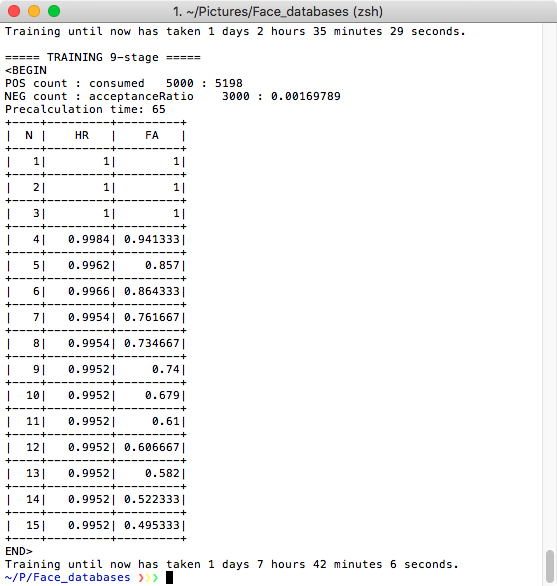
\includegraphics[width=0.95\linewidth]{imagens/opencv_traincascade_fim.png}
    \caption{Fim}\label{fig:opencv_traincascade:b}
    \end{subfigure}
\end{figure}

O treinamento pode demorar vários dias dependendo das especificações do computador e dos parâmetros passados para o comando \texttt{opencv\_traincascade}.
Como visto na \autoref{fig:opencv_traincascade}, o treinamento de um classificador em cascata de 10 estágios utilizando 5000 imagens positivas e 3000 imagens negativas com 36$\times$36 pixels cada demorou 1 dia 7 horas e 42 minutos para ser concluído em um MacBook Air de 2013 com processador Intel Core i5 de 1,3 GHz e 4 GB de RAM.


\section{Uso do classificador}\label{sec:uso_classificador}

Como resultado do treinamento, um arquivo chamado \texttt{cascade.xml} é criado no diretório especificado. Esse arquivo é o classificador em cascata treinado.
Ele pode ser carregado com o método \texttt{cv2.CascadeClassifier} do OpenCV, como usado no \autoref{cod:detector_facial_opencv}, cuja execução pode ser vista na \autoref{fig:detector_facial} e na \autoref{fig:detector_facial_lfw}.

Pela \autoref{fig:detector_facial_lfw}, é possível perceber que o classificador em cascata foi capaz de detectar faces com alguma oclusão, levemente rotacionadas e com expressões, porém o número de falso-positivos foi consideravelmente alto. Este resultado sugere que o classificador deve ser treinado com mais imagens negativas, mais estágios e com um valor menor para o parâmetro maxFalseAlarmRate.

\begin{figure}[htbp]
    \caption{Captura de tela do \autoref{cod:detector_facial_opencv} em execução.}
    \label{fig:detector_facial}
    \begin{center}
        {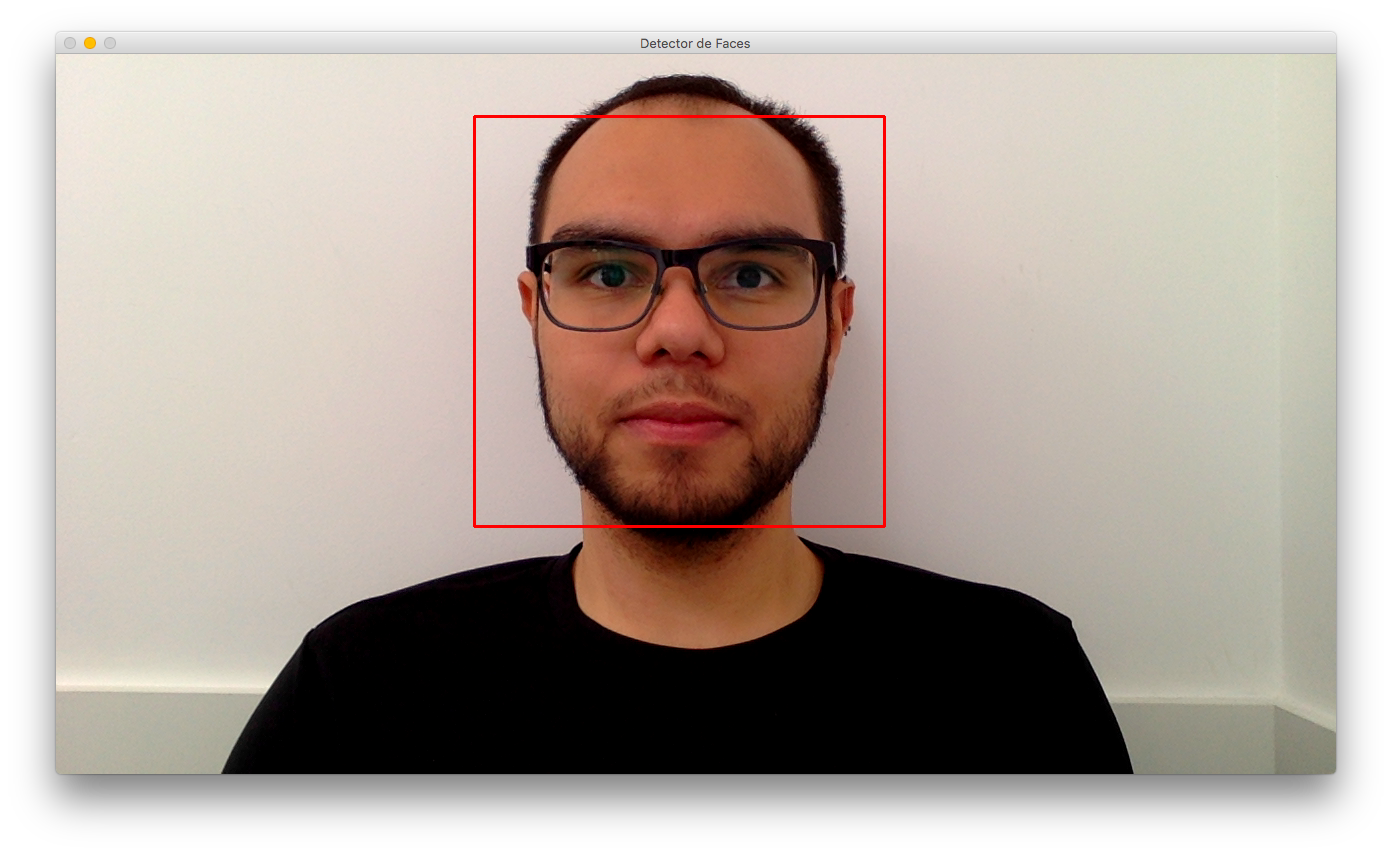
\includegraphics[width=0.55\linewidth]{imagens/detector_facial.png}}
    \end{center}
\end{figure}

\begin{figure}[htbp]
    \caption{Teste do classificador em cascata com imagens da Labeled Faces in the Wild}
    \label{fig:detector_facial_lfw}
    \begin{center}
        {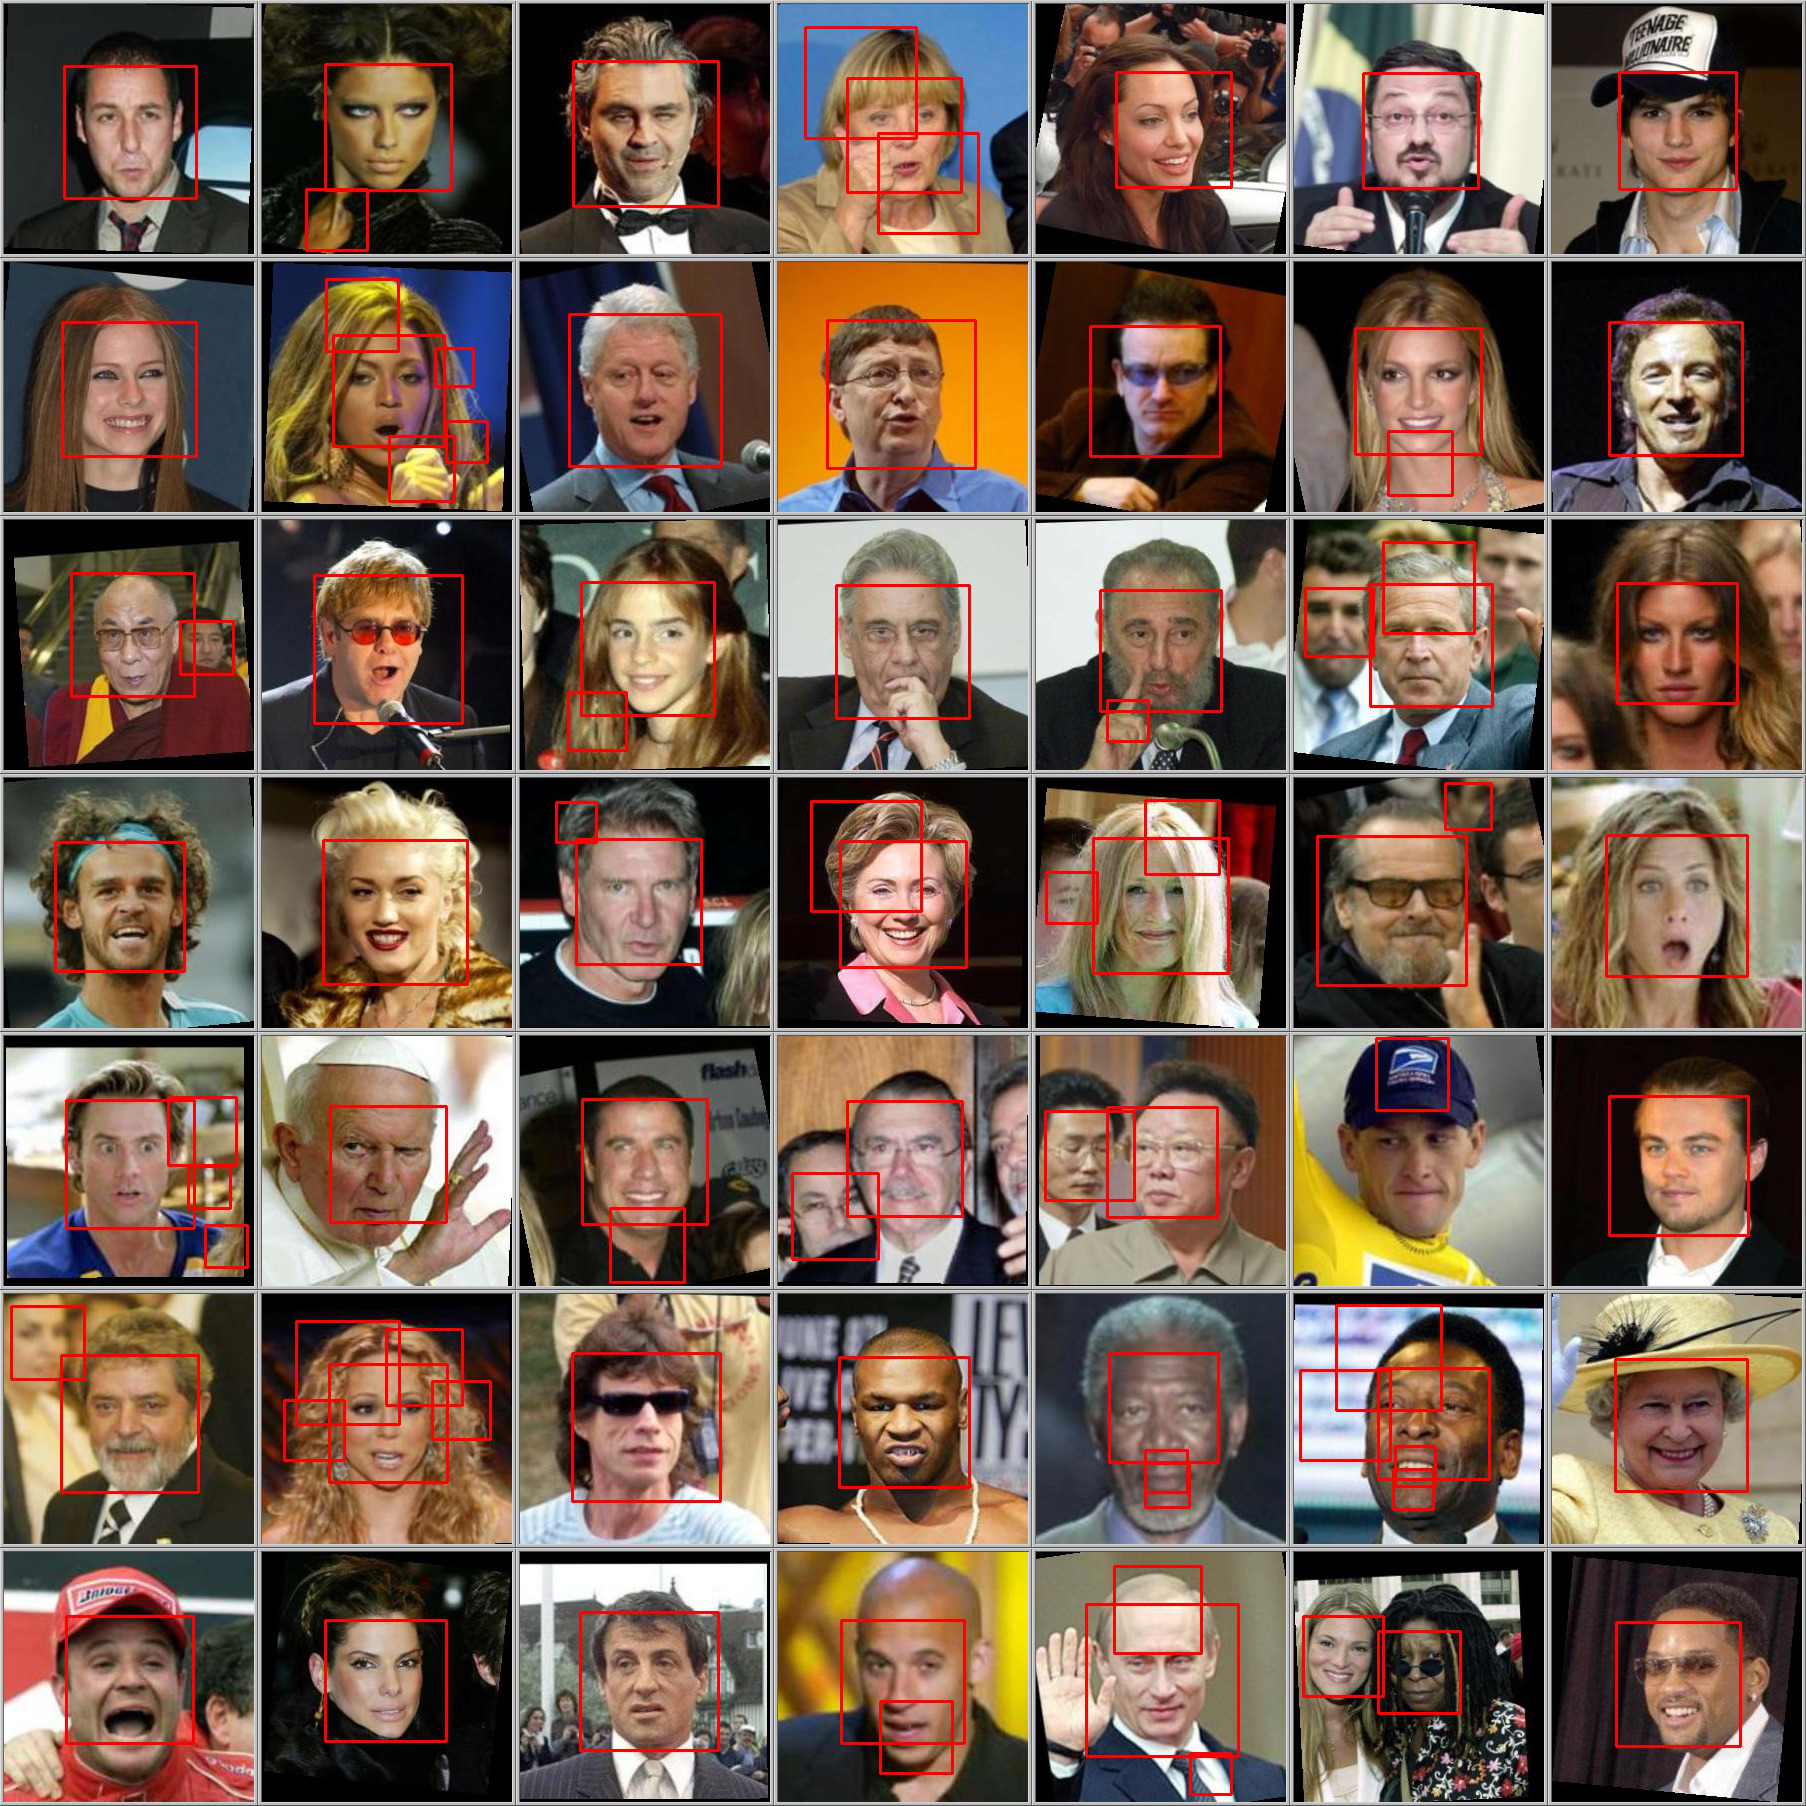
\includegraphics[width=0.95\linewidth]{imagens/detector_facial_lfw.jpg}}
    \end{center}
\end{figure}

% ----------------------------------------------------------
% PARTE
% ----------------------------------------------------------
\part{Reconhecimento Facial}

% ----------------------------------------------------------
% Capitulo 4
% ----------------------------------------------------------
\chapter{Reconhecimento facial}\label{cap:reconhecimento_facial}

Um sistema de reconhecimento facial é uma tecnologia capaz de realizar identificação ou verificação automática de uma pessoa através de uma imagem ou vídeo. 

Segundo \citeonline{jafri2009survey}, essas duas tarefas principais do reconhecimento facial podem ser definidas como:
%
\begin{itemize}
\item \textbf{Verificação} (correspondência um-para-um): dada uma face e uma alegação de identidade, informa se a face realmente pertence ao indivíduo.  

\item \textbf{Identificação} (correspondência de um-para-muitos): compara a imagem de uma face desconhecida com todas as imagens em um banco de dados para determinar sua identidade.
\end{itemize}

Uma terceira tarefa também importante é a de agrupamento (clustering), que consiste em agrupar faces da mesma pessoa mesmo que essa pessoa não esteja cadastrada em um banco. \cite{dhingra2017face, schroff2015facenet}.

São várias as aplicações práticas desses sistemas, como autenticação biométrica, vigilância, interação humano-computador e gerenciamento multimídia. \cite{jain2011handbook}.

O reconhecimento facial possui diversas vantagens sobre outras formas de biometria. Para validação de passaportes, por exemplo, \citeonline{heitmeyer2000biometric} afirma que esse é o método preferido por ser rápido, não intrusivo e poder ser feito à distância sem necessidade de contato.

A tarefa de verificação facial em cenários cooperativos, nos quais as condições de iluminação e pose são controladas, já pode ser considerada um problema bem resolvido. Por outro lado, a identificação um-para-muitos, especialmente em cenários não cooperativos, como busca por pessoas desaparecidas ou procuradas pela polícia, ainda é uma tarefa desafiadora.
A performance do reconhecimento é grandemente influenciada por variações nas condições de iluminação, ponto de vista, poses, expressão facial, envelhecimento, uso de disfarces e acessórios \cite{li2016kernel, jain2011handbook}.

Dentre os trabalhos pioneiros em reconhecimento facial automatizado, destacam-se a tese de doutorado de Takeo Kanade em \citeyear{kanade1973picture}, os trabalhos sobre representação de faces em dimensionalidade reduzida usando PCA feitos por Kirby e Sirovich em \citeyear{sirovich1987low} e \citeyear{kirby1990application} e os trabalhos sobre Eigenfaces de Turk e Pentland em \citeyear{turk1991eigenfaces}.

Outras técnicas relevantes utilizam discriminantes lineares (Fisherfaces LDA) \cite{belhumeur1997eigenfaces, etemad1996face}, local binary patterns (LBP) \cite{ojala1994performance}, filtros de Gabor \cite{lades1993distortion, wiskott1997face, gonccalves2016robusto} e, mais recentemente, GaussianFace (DGP-LVM) \cite{lu2015surpassing} e redes neurais profundas (DNN) \cite{taigman2014deepface, he2015delving, sun2014deep, sun2014predict, sun2015deeply, zhu2014recover, schroff2015facenet, zhou2015naive, yi2014learning, sun2015deepid3, amos2016openface}.

Redes neurais profundas podem ser consideradas o estado da arte em reconhecimento facial. Com taxas de detecção acima de 99,8\% na LFW, esses métodos já ultrapassam a performance humana nesse teste \cite{learned2016labeled, kumar2009attribute}.

O processo de reconhecimento automático de faces envolve três etapas: detecção de faces, extração de características e identificação ou verificação, como ilustrado na \autoref{fig:etapas_reconhecimento}. Na fase de extração de características, é comum realizar uma normalização para alinhar as faces.

\begin{figure}[htbp]
    \caption{Etapas do reconhecimento facial}
    \label{fig:etapas_reconhecimento}
    \begin{adjustbox}{max width=\textwidth}
    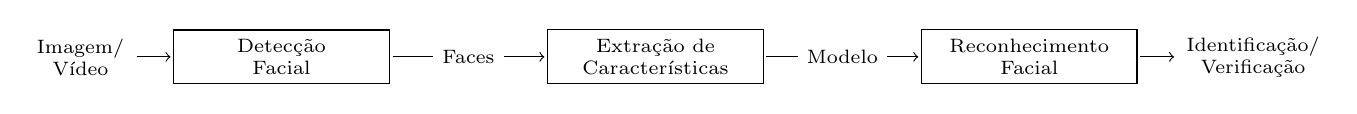
\begin{tikzpicture}[
        font=\scriptsize, node distance=2cm,
        mynode/.style={draw, text width=2.5cm, align=center}
        ]
        \node[align=center] (input) {Imagem/\\Vídeo};
        \node[mynode,right=0.5cm of input] (detec) {Detecção\\Facial};
        \node[mynode,right=of detec] (extra) {Extração de\\Características};
        \node[mynode,right=of extra] (recon) {Reconhecimento\\Facial};
        \node[align=center,right=0.5cm of recon] (ident) {Identificação/\\Verificação};
        
        \draw[->,shorten <=1pt,shorten >=1pt] (input) -- (detec);
        \draw[->,shorten <=1pt,shorten >=1pt] (detec) -- node[fill=white] {Faces}(extra);
        \draw[->,shorten <=1pt,shorten >=1pt] (extra) -- node[fill=white] {Modelo}(recon);
        \draw[->,shorten <=1pt,shorten >=1pt] (recon) -- (ident);
    \end{tikzpicture}
    \end{adjustbox}
\end{figure}

Os algoritmos Eigenfaces, Fisherfaces e Local Binary Patterns Histograms (LBPH) estão implementados na biblioteca OpenCV \cite{opencvreconhecimento}.


\section{Extração de características}\label{sec:extract_caract}

Imagens digitais são representadas por milhares de pixels que são codificados em arrays de alta dimensionalidade. Os métodos de extração de características procuram encontrar as informações mais relevantes das imagens originais e representá-las em um espaço de menor dimensionalidade.

Existem $256^{10000}$ formas diferentes de formar uma imagem em tons de cinza (8 bits) de $100\times100$ pixels, mas apenas uma pequena fração dessas imagens representam faces. Além disso, muitas características são comuns a todas as faces e não são úteis para diferenciá-las.

A redução da dimensionalidade do espaço permite eliminar essas redundâncias e características indesejadas. Ela pode ser realizada se o erro quadrático médio (EQM) ou a soma da variância dos elementos forem mínimas, o que é verdade para imagens de faces por elas compartilharem muitas similaridades.

%%%% TODO: Talvez mover para eigenfaces?
Como explicado por \citeonline{datta2015face}, a ideia principal dos métodos de reconhecimento facial baseados em subespaço é encontrar vetores que melhor representam a distribuição de faces em todo o espaço da imagem. Esses vetores de dimensão reduzida definem o subespaço das faces. Após a linearização, o vetor médio entre todas as imagens de faces é calculado e subtraído de cada vetor correspondente às faces originais. Depois, a matriz de covariância é calculada para extrair um número limitado de autovetores, correspondentes aos maiores autovalores. Esses autovetores, também chamados eigenfaces, representam uma base em um espaço de baixa dimensionalidade. Para testar uma imagem, sua eigenface é calculada e comparada com todas as faces no banco de dados.

Os principais métodos que utilizam subespaços para reconhecimento facial são o PCA e o LDA \cite{wang2004unified}. O PCA seleciona as características que melhor representam a face e o LDA seleciona o subespaço que melhor discrimina classes de faces. Eles também podem ser utilizados em conjunto.


\subsection{Análise de componentes principais (PCA)}\label{sec:pca}

A análise de componentes principais (em inglês, principal component analysis ou PCA) é uma técnica de redução de dimensionalidade inventada em 1901 por \citeonline{pearson1901liii}.
Em \cite{gerbrands1981relationships} foi concluído que PCA é o mesmo que a transformada de Karhunen-Loève (KLT) exceto por uma possível mudança na origem do sistema de coordenadas.
Em \cite{andrews1975two} foi alertado que, apesar de próximos, SVD (decomposição em valores singulares) não é o mesmo que PCA e KLT. 

\begin{figure}[htbp]
    \caption{Análise de Componentes Principais}
    \label{fig:pca}
    \begin{subfigure}[c]{0.45\textwidth}
    \centering
    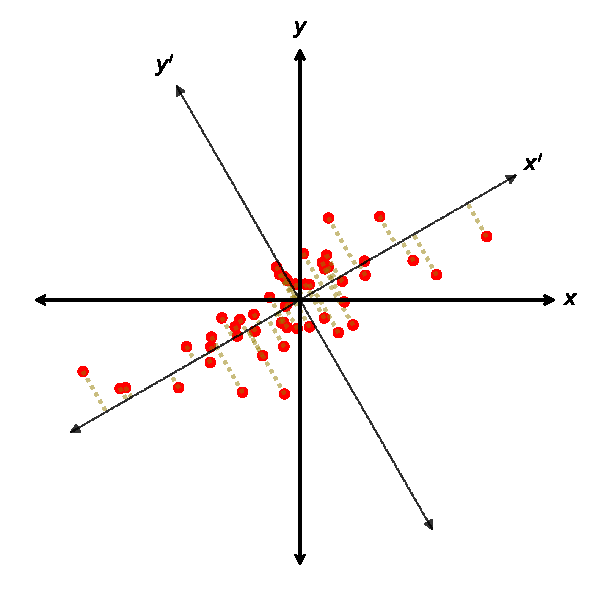
\includegraphics[width=\textwidth]{imagens/pca1.pdf}
    \caption{Distribuição original}
    \end{subfigure}
    \begin{subfigure}[c]{0.45\textwidth}
    \centering
    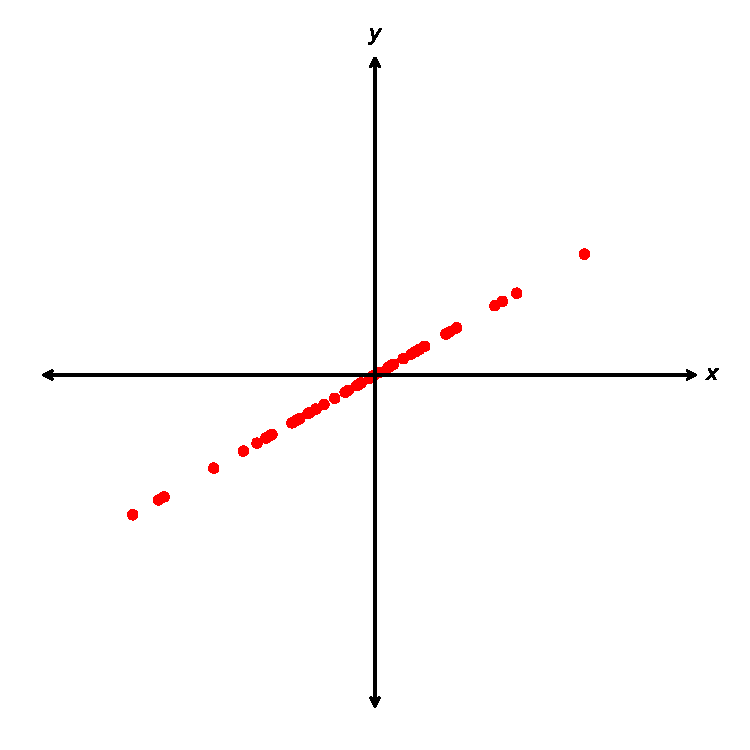
\includegraphics[width=\textwidth]{imagens/pca2.pdf}
    \caption{Apenas o primeiro componente principal}
    \end{subfigure}
\end{figure}

Segundo \cite{jolliffe2002principal}, a ideia central da análise de componentes principais (PCA) é reduzir a dimensionalidade de um conjunto de dados que consiste em um grande número de variáveis, mantendo o máximo possível da variação presente no conjunto de dados. Isto é alcançado através da transformação para um novo conjunto de variáveis, os componentes principais, que não são correlacionados e são ordenados de forma que os primeiros retenham a maior parte da variação presente em todas as variáveis originais.

O conceito do PCA está ilustrado na \autoref{fig:pca}. Os eixos $x$ e $y$ formam a base original e o eixo $x'$ corresponde à direção de maior variância, ou seja, ao primeiro componente principal.

Matematicamente, dados $n$ pontos em $\mathbb{R}^p$, a PCA consiste em escolher uma dimensão $k < p$ e encontrar um espaço afim de dimensão $k$ onde a distância ao quadrado dos pontos às suas projeções ortogonais no espaço são minimizadas.


\subsection{Eigenfaces}\label{sec:eigenfaces}

As eigenfaces são os componentes principais de uma distribuição de faces, ou seja, os autovetores da matriz de covariância de um conjunto de imagens de faces.
Cada face pode ser representada como uma combinação linear de eigenfaces, como mostra a \autoref{fig:eigenfaces_comblinear}. Elas também podem ser aproximadas usando apenas as eigenfaces que possuem os maiores autovalores e que, consequentemente, são responsáveis pela maior variância.

A ideia de usar componentes principais para representar faces humanas foi desenvolvida por \citeonline{sirovich1987low} e usada por \cite{turk1991eigenfaces} para detecção e reconhecimento facial.
Muitos consideram essa técnica de reconhecimento facial baseada em aparência como a primeira a ser utilizada com sucesso na prática.

\begin{figure}[htbp]
    \centering
    \caption{Representação de uma face como combinação linear de eigenfaces}
    \label{fig:eigenfaces_comblinear}
    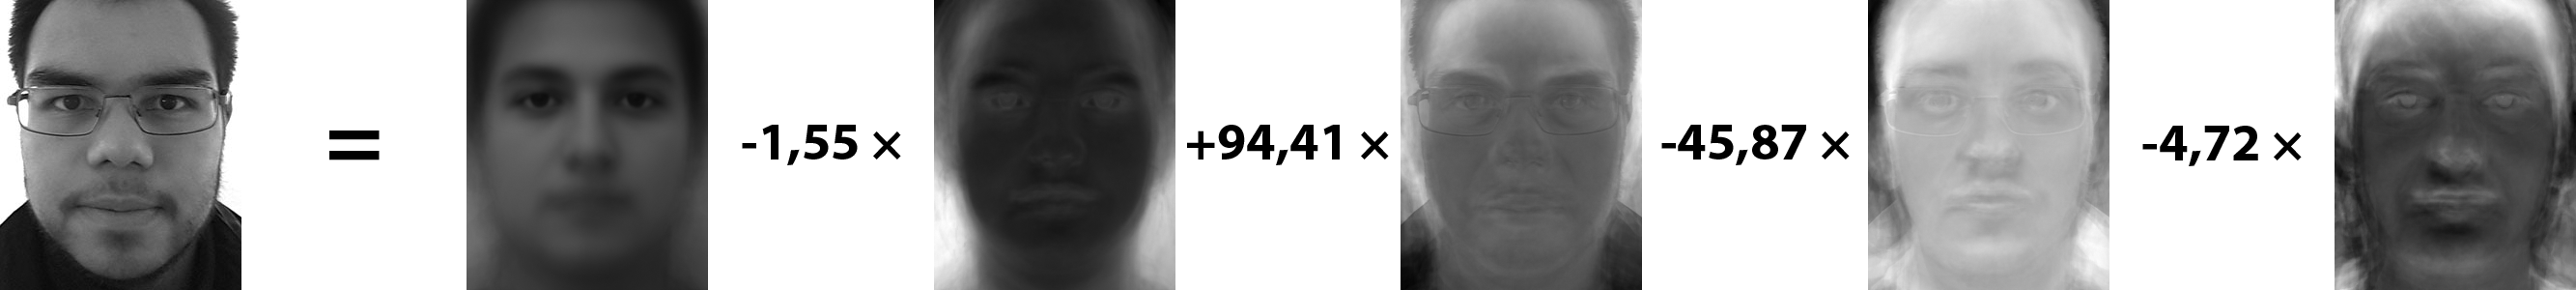
\includegraphics[width=0.95\linewidth]{imagens/eign_lincomb.png}
\end{figure}


\subsubsection{Algoritmo para cálculo das eigenfaces}\label{sec:eigenfaces_algoritmo}

O algoritmo para a obtenção das eigenfaces proposto por \citeonline{turk1991face} pode ser formulado da seguinte forma:

\begin{enumerate}
    \item Obter $M$ imagens $I_1, I_2, I_3 \ldots I_M$ com dimensão $N \times N$.
    As imagens devem estar centralizadas.
    \item Representar cada imagem $I_i$ como um vetor $\Gamma_i$ de dimensão $N^2 \times 1$.
    %
    \begin{equation} \label{eq:eign_gamma}
        \begin{bmatrix}
        a_{11} & a_{12} & \cdots & a_{1N}\\ 
        a_{21} & a_{22} & \cdots & a_{2N}\\ 
        \vdots & \vdots & \ddots & \vdots\\ 
        a_{N1} & a_{N1} & \cdots & a_{NN}
        \end{bmatrix}_{N \times N} \rightarrow \begin{bmatrix}
        a_{11}\\ 
        \vdots\\ 
        a_{1N}\\ 
        \vdots\\ 
        a_{2N}\\
        \vdots\\ 
        a_{NN}
        \end{bmatrix}_{N^2 \times 1}
    \end{equation}
    %
    \item Calcular o vetor $\Psi$ correspondente à face média.
    %
    \begin{equation} \label{eq:eign_media}
        \Psi = \frac{1}{M}\sum_{i=1}^{M}\Gamma_i
    \end{equation}
    %
    \item Subtrair a face média de cada vetor $\Gamma_i$ para obter o conjunto de vetores $\Phi_i$.
    %
    \begin{equation} \label{eq:eign_phi}
        \Phi_i = \Gamma_i - \Psi
    \end{equation}
    %
    \item Encontrar a matriz $C$ de covariância.
    %
    \begin{equation} \label{eq:eign_c}
        C = AA^T \text{, onde } A = \begin{bmatrix}\Phi_1  & \Phi_2 & \ldots  & \Phi_3\end{bmatrix}
    \end{equation}
    %
    $C$ é uma matriz $N^2 \times N^2$ e $A$ é uma matriz $N^2 \times M$.
    \item Calcular os autovetores $u_i$ de $C = AA^T$.
    
    Em vez desse cálculo, que resultaria em $N^2$ autovetores, calcular os autovetores $v_i$ da matriz $A^TA$ de dimensão $M \times M$.
    %
    \begin{equation} \label{eq:eign_autov}
    \begin{alignedat}{2}
                     && A^T Av_i    &= \mu_i v_i\\
    \Rightarrow\quad && AA^T Av_i   &= \mu_i Av_i\\
    \Rightarrow\quad && CAv_i       &= \mu_i Av_i\\
    \Rightarrow\quad && u_i         &= Av_i
    \end{alignedat}
    \end{equation}
    %
    ou seja, $Av_i$ são autovetores de $C = AA^T$. Os $M$ autovalores de $A^TA$ correspondem aos $M$ maiores autovalores de $AA^T$.
    \item Manter apenas os $K$ autovetores, correspondentes aos $K$ maiores autovalores.
\end{enumerate}

Cada face $\Phi_i$ (face menos a média), correspondente a uma das $M$ imagens de treinamento, possui uma representação vetorial $\Omega_i$ na base formada pelos $K$ autovetores escolhidos, ou seja, pode ser representada pela seguinte combinação linear:
%
\begin{equation} \label{eq:eign_lincomb}
    \Gamma_i - \Psi = \Phi_i = \sum_{j=1}^{K}w_ju_j, (w_j = u_{j}^{T}\Phi_i)
\end{equation}
%
Cada peso $w_j$ descreve a contribuição do autovetor $u_j$ na representação da imagem. Eles formam o seguinte vetor $\Omega_i$:
%
\begin{equation} \label{eq:eign_lincomb_vetor}
\Omega_i = \begin{bmatrix}
        w_{1}^{i}\\ 
        w_{2}^{i}\\ 
        \vdots\\ 
        w_{K}^{i}
        \end{bmatrix}, i = 1, 2, \ldots, M
\end{equation}
%

\subsubsection{Reconhecimento usando eigenfaces}\label{sec:eigenfaces_reconhecimento}

O reconhecimento de uma face desconhecida $\Gamma$ centralizada e com as mesmas dimensões das imagens de treinamento é feito através dos seguintes passos:

\begin{enumerate}
    \item Normalização da imagem.
        \begin{equation} \label{eq:eign_rec_norm}
            \Gamma: \Phi = \Gamma - \Psi
        \end{equation}
    \item Projeção no autoespaço.
        \begin{equation} \label{eq:eign_rec_lincomb}
            \hat{\Phi} = \sum_{i=1}^{K}w_iu_i, (w_i = u_{i}^{T}\Phi)
        \end{equation}
    \item Representação de $\Phi$ como $\Omega$:
        \begin{equation} \label{eq:eign_rec_omg}
            \Omega = \begin{bmatrix}
            w_{1}\\ 
            w_{2}\\ 
            \vdots\\ 
            w_{K}
            \end{bmatrix}
        \end{equation}
    \item Cálculo da distância (euclidiana) mínima $e_r = min_l\left \| \Omega - \Omega^l \right \|$.
    \item Se a distância $e_r$ foi menor que um limite $T_r$ escolhido, então $\Gamma$ é reconhecida como a face l do conjunto de treino.
\end{enumerate}


\begin{figure}[htbp]
    \centering
    \caption{Eigenfaces}
    \label{fig:eigenfaces_faces}
    \begin{subfigure}[t]{0.3\textwidth}
    \centering
    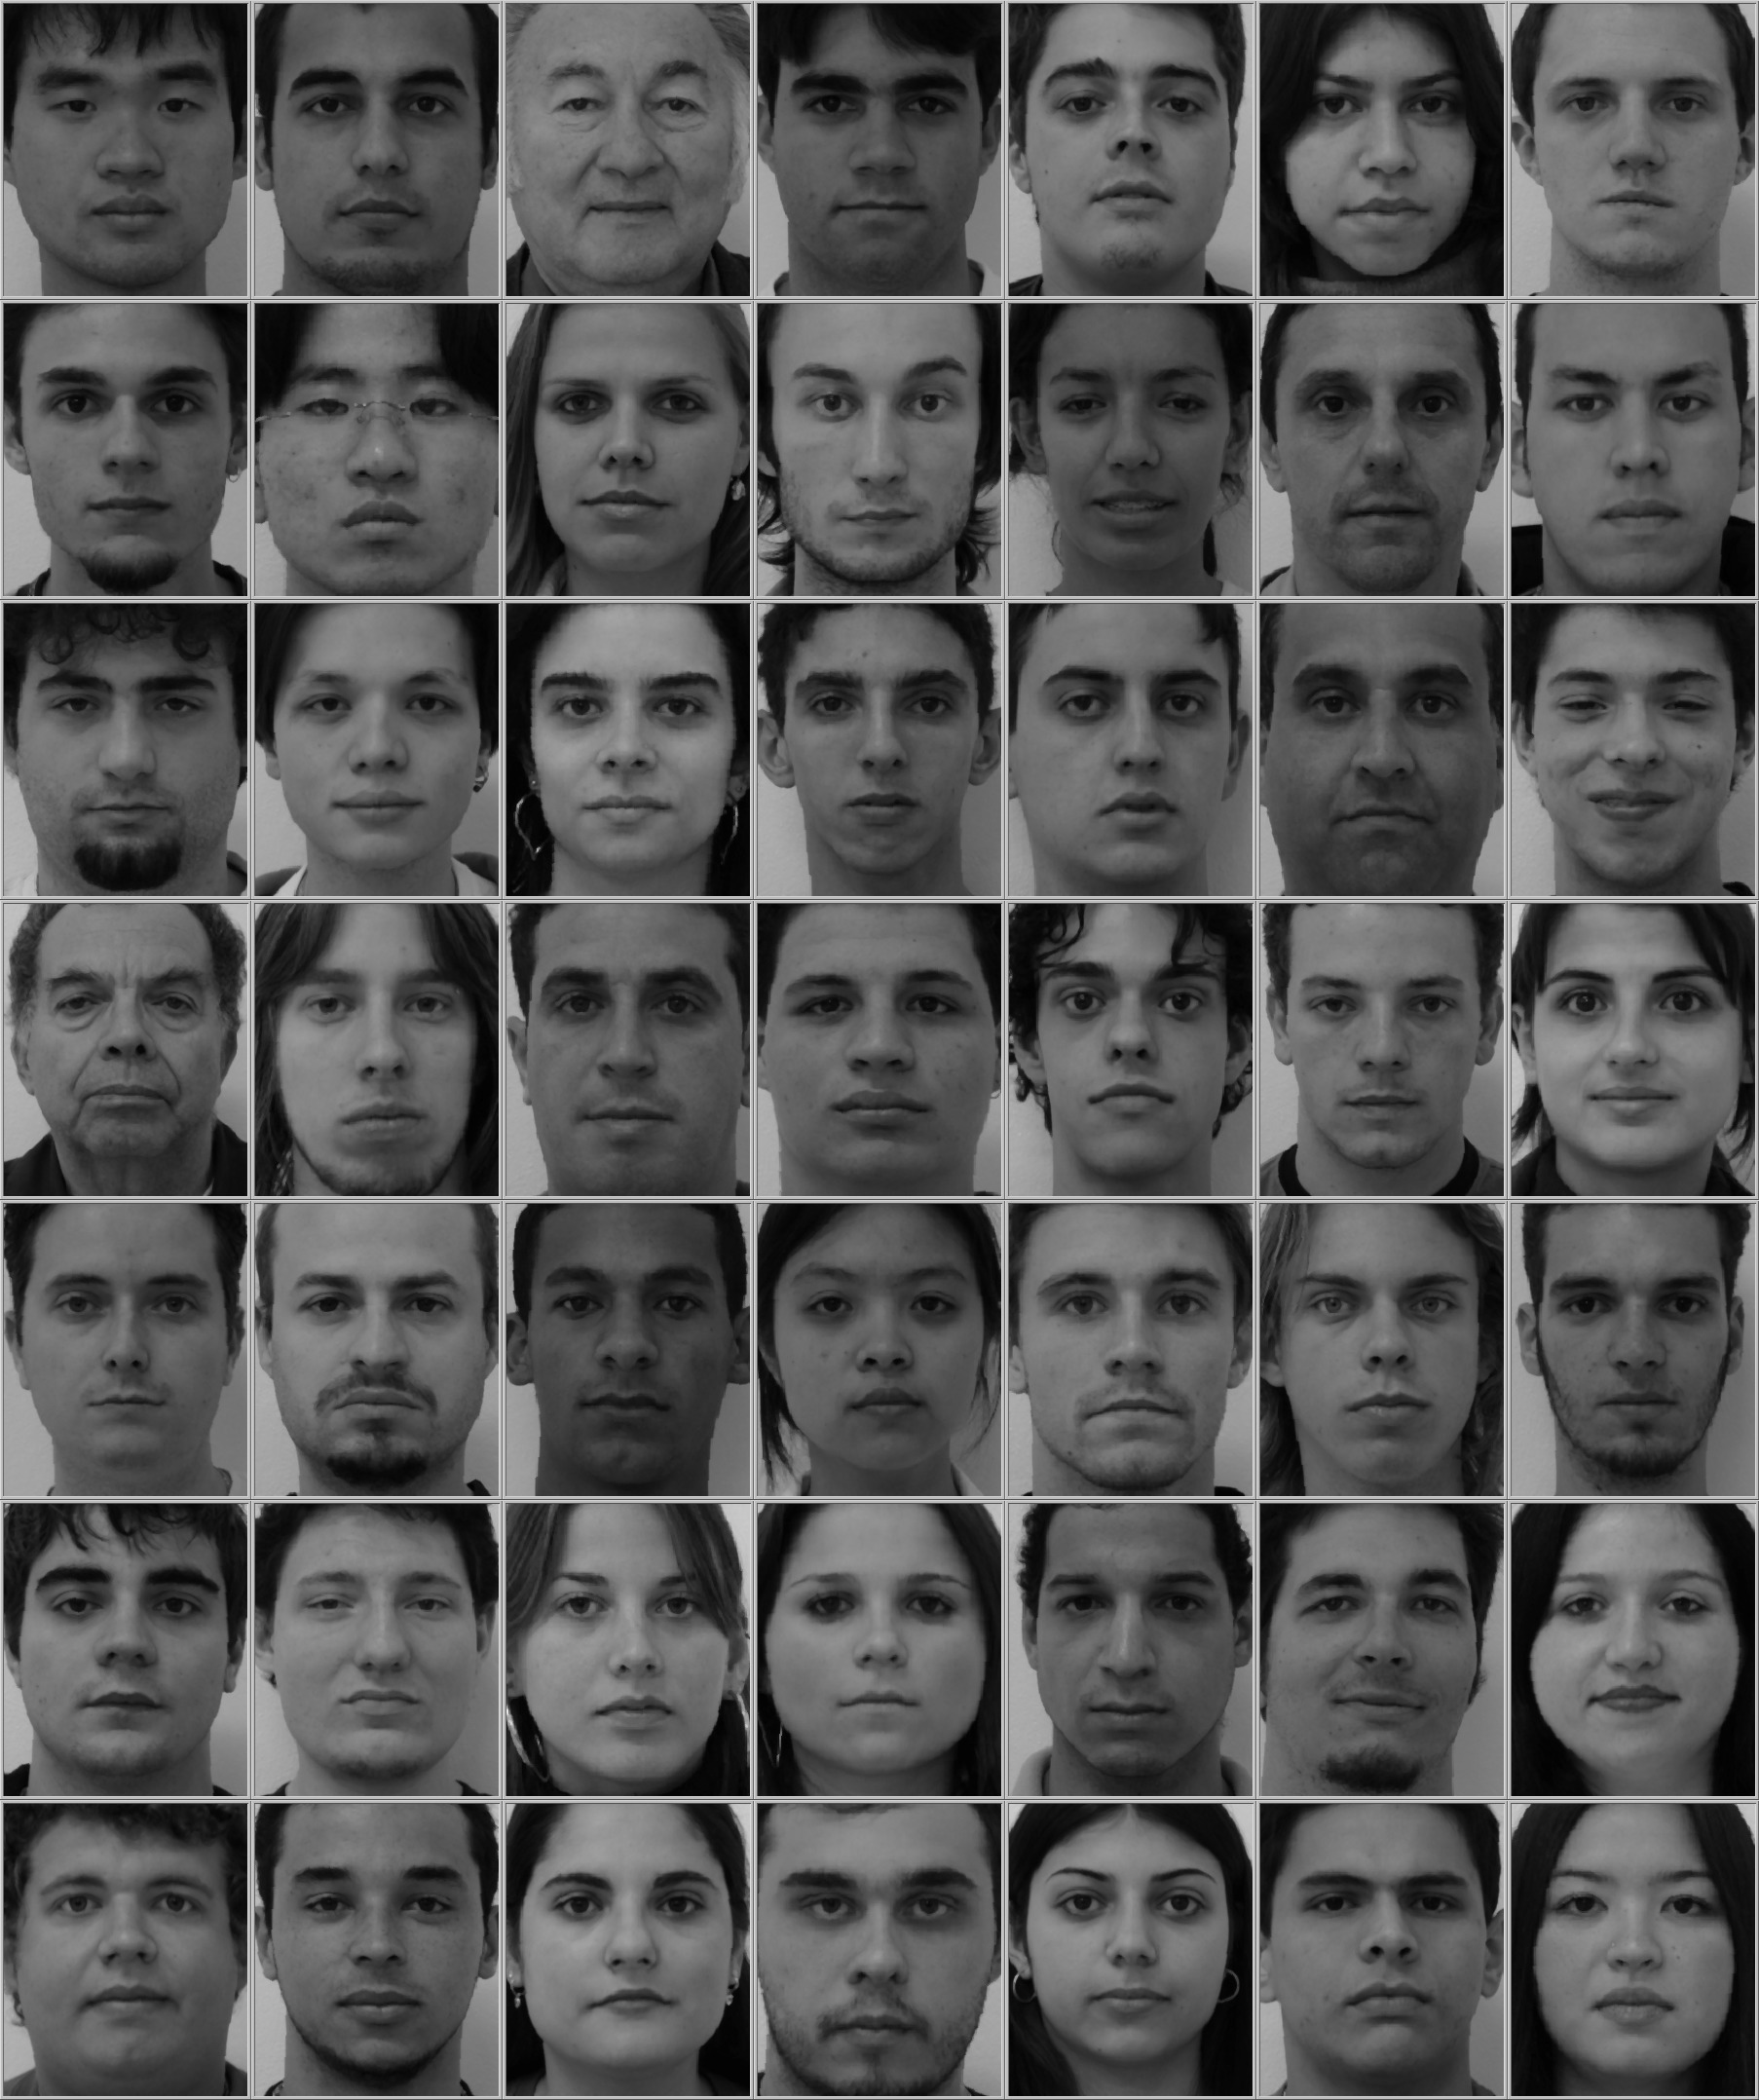
\includegraphics[width=\textwidth]{imagens/faces_fei.jpg}
    \caption{Alguma faces da FEI Face Database}
    \end{subfigure}
    \begin{subfigure}[t]{0.3\textwidth}
    \centering
    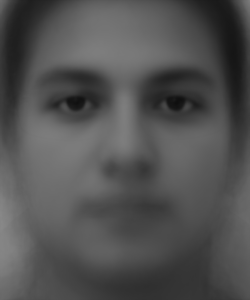
\includegraphics[width=\textwidth]{imagens/face_media.png}
    \caption{Face média}
    \end{subfigure}
    \begin{subfigure}[t]{0.3\textwidth}
    \centering
    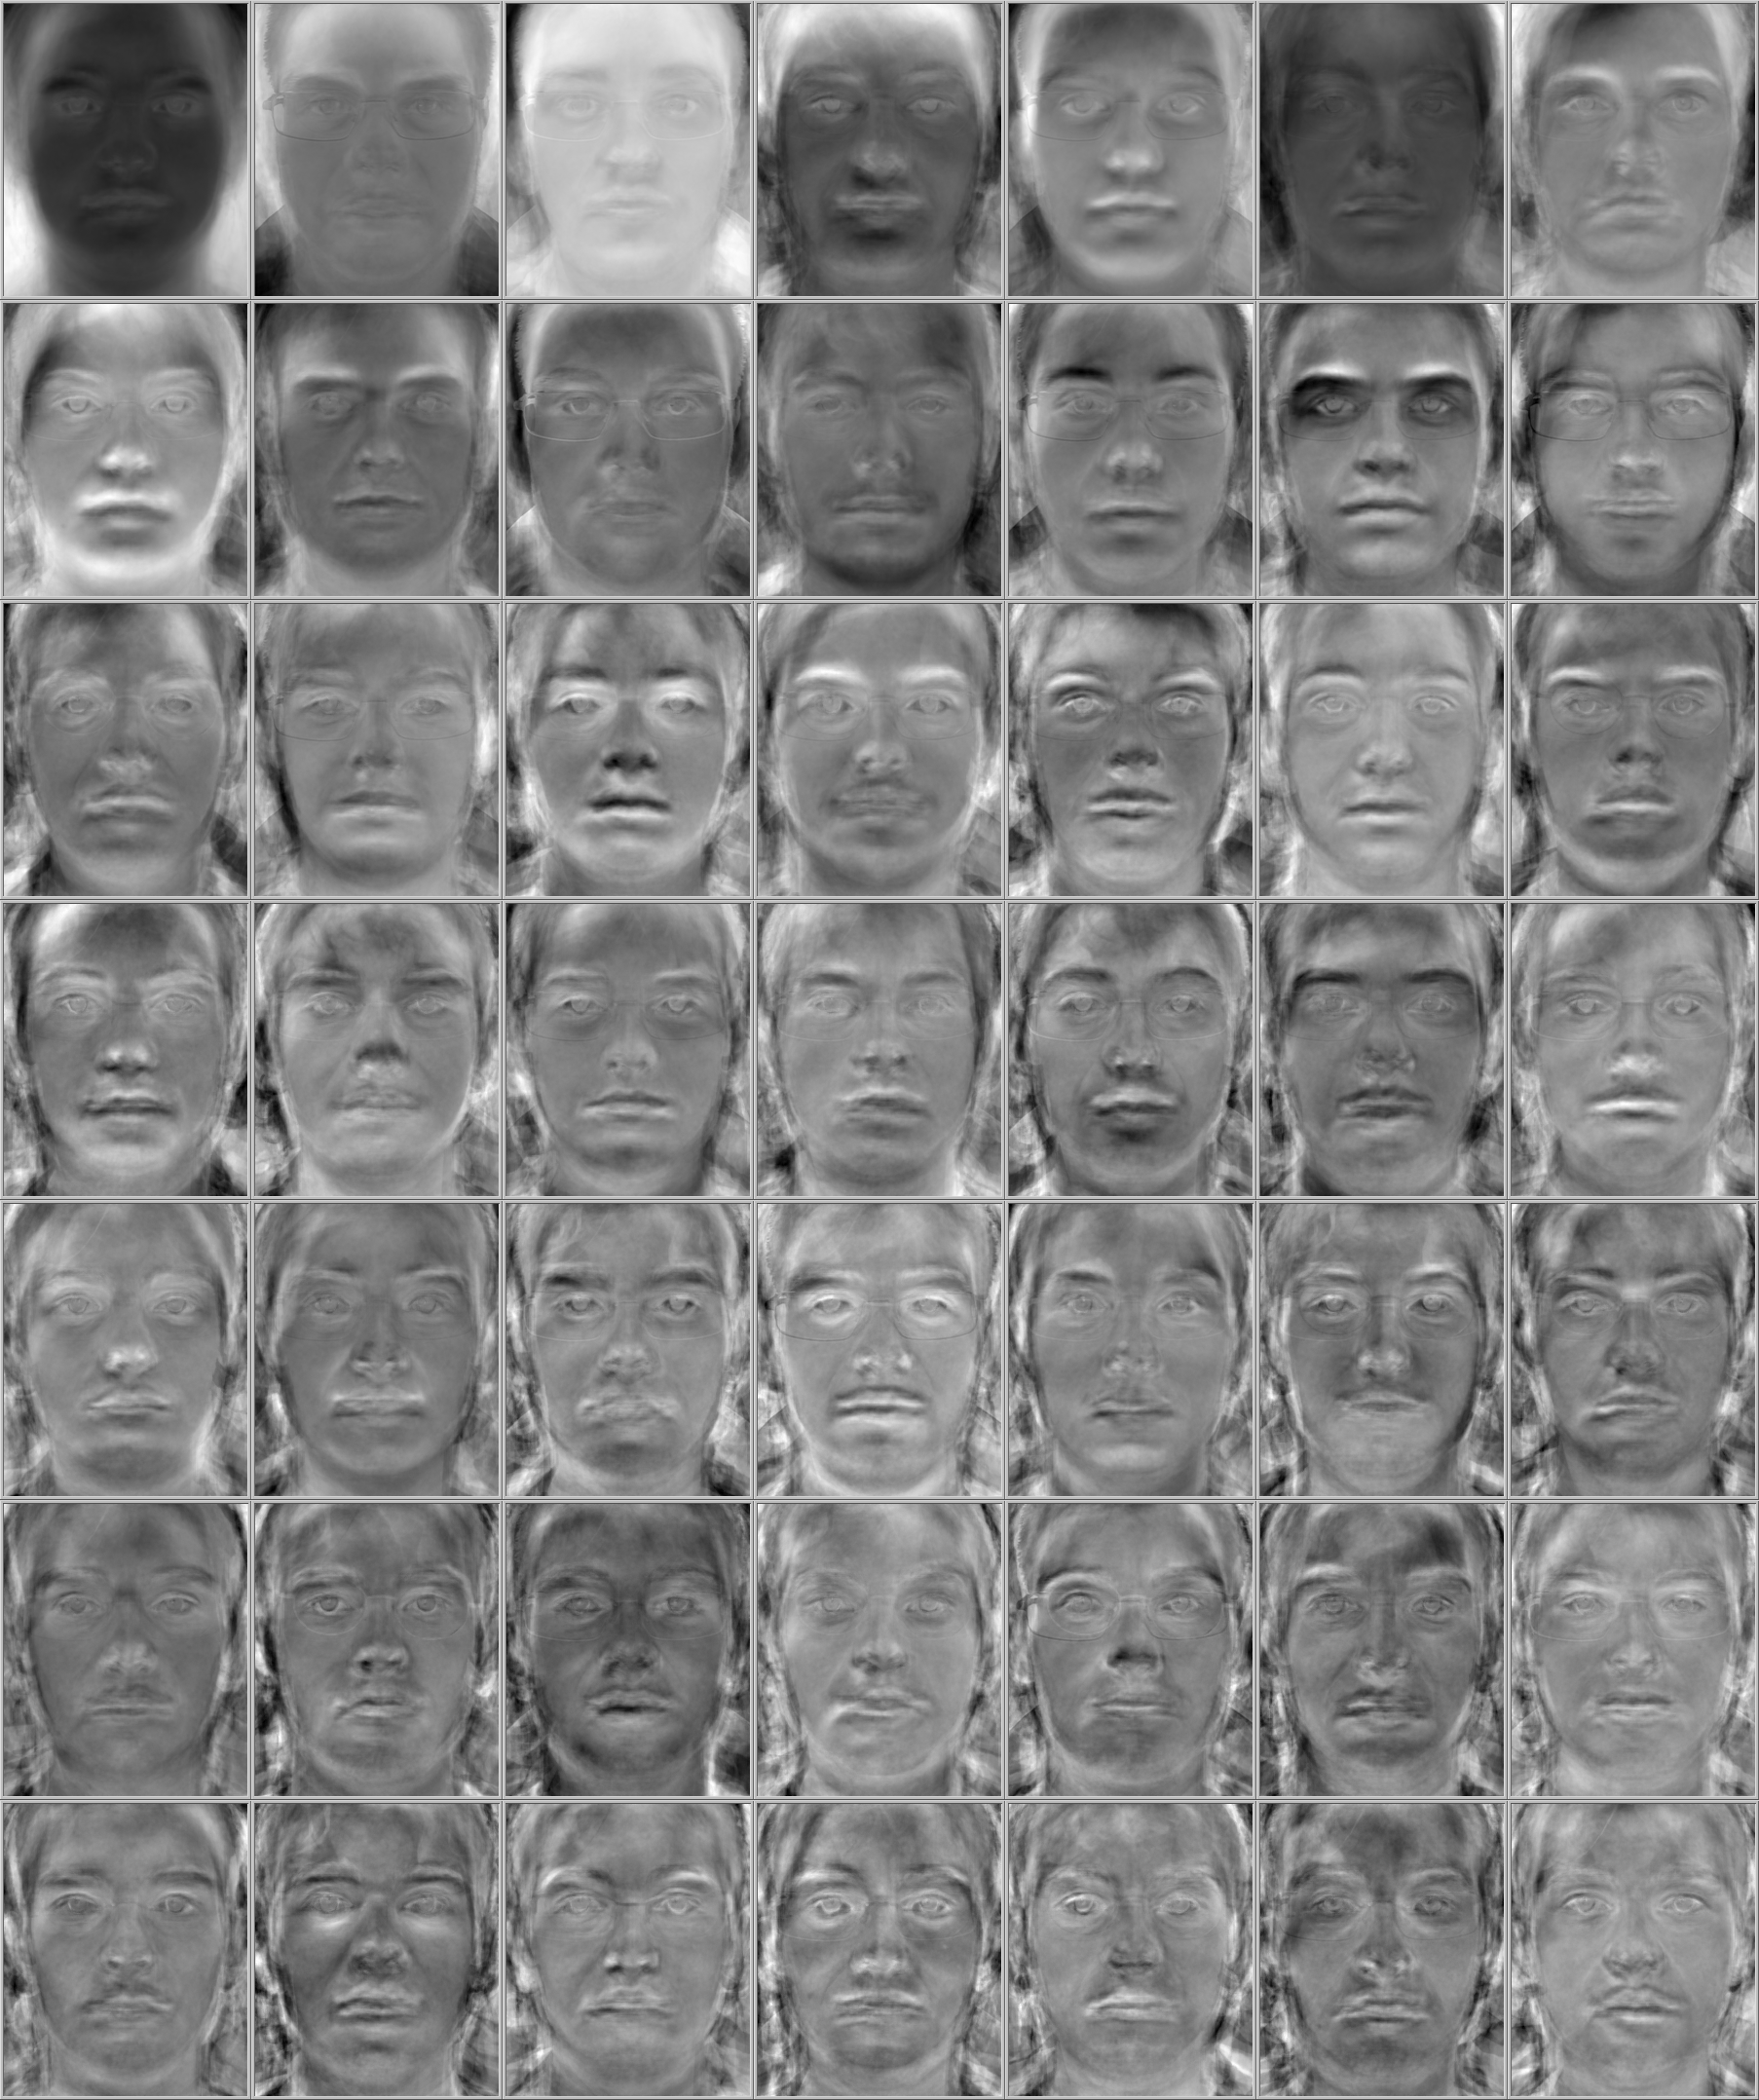
\includegraphics[width=\textwidth]{imagens/eigenfaces.png}
    \caption{Eigenfaces}
    \end{subfigure}
\end{figure}

\subsubsection{Implementação e avaliação do algoritmo}\label{sec:eigenfaces_testes}

O \autoref{cod:eigenfaces_opencv} apresenta como realizar o reconhecimento facial com Eigenfaces utilizando a classe \texttt{EigenFaceRecognizer} da biblioteca OpenCV.

Foram realizados três testes para avaliar o desempenho do algoritmo com diferentes bases de faces. O primeiro utilizou a base da AT\&T, um subconjunto da FERET database foi utilizado para o segundo teste e o terceiro foi feito com algumas imagens selecionadas da Extended Yale Face Database B.

No primeiro teste, foram utilizadas 9 fotos de cada um dos 40 indivíduos para o treino e uma foto de cada para a avaliação.
Das 40 faces de teste, o algoritmo reconheceu 38 faces com sucesso e errou o reconhecimento de duas. A taxa de reconhecimento obtida foi de 95\%, o que sugere que o método das eigenfaces tem bom resultado quando utilizado com imagens frontais de poucas pessoas em ambientes com iluminação controlada. Esse resultado pode ser visto na \autoref{fig:eigenfaces_resultado_att}.

No segundo teste, usando um subconjunto da base de faces FERET composto por 1542 imagens frontais de 865 pessoas para treino e uma foto de avaliação para cada pessoa, o algoritmo obteve 550 acertos e 315 erros, ou seja, uma taxa de apenas 63,6\% de acertos mesmo com pose e iluminação controladas. Isso se deve, provavelmente, pelo grande número de indivíduos e pelo baixo número de imagens de treino por indivíduo.

No terceiro teste, foram utilizadas 49 imagens de cada um dos 38 indivíduos para treinamento e uma foto de cada para testar o reconhecimento. O algoritmo obteve 31 acertos e 7 erros, ou seja, 81,6\% de acertos. Esse resultado está exposto na \autoref{fig:eigenfaces_resultado_yale}.

O reconhecimento facial com eigenfaces é muito vulnerável a mudanças na iluminação e na orientação da face. Em \cite{baggio2012mastering} são dadas algumas sugestões de pré-processamento, ilustradas na \autoref{fig:preprocessamento}, que ajudam a diminuir o impacto desses fatores:
%
\begin{itemize}
    \item \textbf{Transformações geométricas}: redimensionar, rotacionar e transladar a imagem de forma que os olhos fiquem alinhados.
    
    \item \textit{\textbf{Cropping}}: remoção da testa, queixo, orelhas e fundo da imagem.
    
    \item \textbf{Equalização do histograma}: deve ser feito para ambos os lados da face para ajustar o brilho e o contraste em cada lado de forma independente.
    
    \item \textbf{Suavização usando filtros bilaterais}: esse processo reduz o ruído da imagem.
    
    \item \textbf{Máscara elíptica}: máscara que contorna a face a fim de remover o cabelo e o fundo da imagem.
\end{itemize}

\begin{figure}[ht]
    \centering
    \caption[Pré-processamentos para melhorar reconhecimento]{Pré-processamentos sugeridos por \citeonline{baggio2012mastering} para melhorar a performance dos algoritmos de reconhecimento facial}
    \label{fig:preprocessamento}
    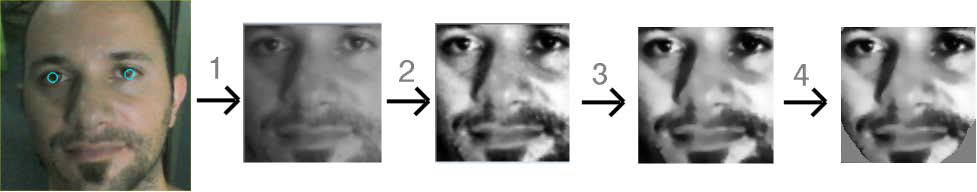
\includegraphics[width=0.95\linewidth]{imagens/preprocessamento.png}
\end{figure}

\begin{figure}[htbp]
    \centering
    \caption[Teste do algoritmo Eigenfaces - AT\&T]{Teste do reconhecimento usando Eigenfaces com a base de faces da AT\&T. Em verde as detecções corretas, em vermelho as erradas}
    \label{fig:eigenfaces_resultado_att}
    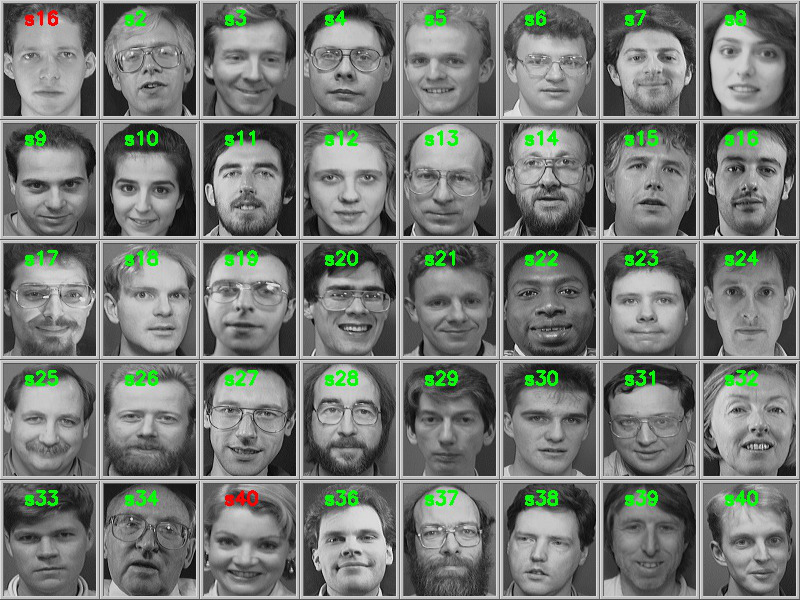
\includegraphics[width=0.8\linewidth]{imagens/eigenfaces_resultado_att.jpg}
    \vspace{\floatsep}
    \caption[Teste do algoritmo Eigenfaces - FERET]{Teste do reconhecimento usando Eigenfaces com a base de faces FERET. Em verde as detecções corretas, em vermelho as erradas}
    \label{fig:eigenfaces_resultado_feret}
    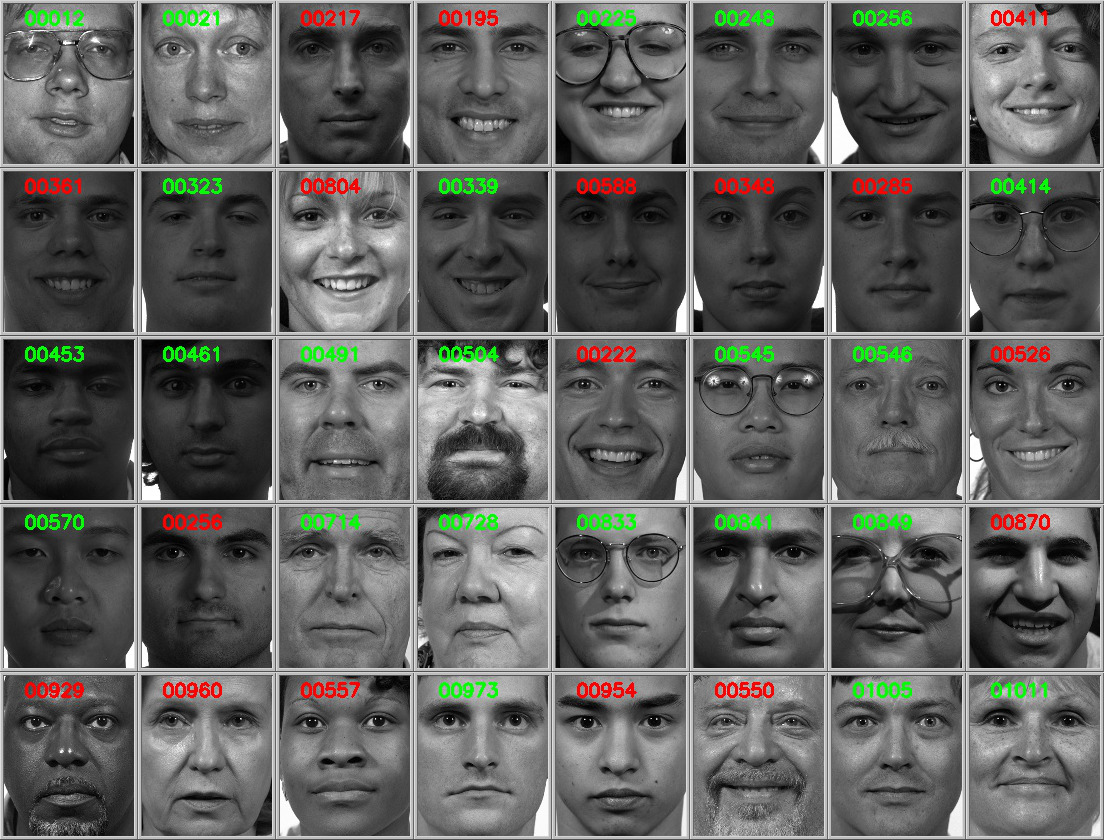
\includegraphics[width=0.8\linewidth]{imagens/eigenfaces_resultado_feret.jpg}
\end{figure}

\begin{figure}[htbp]
    \centering
    \caption[Teste do algoritmo Eigenfaces - Yale]{Teste do reconhecimento usando Eigenfaces com o Extended Yale Face Database B. Em verde as detecções corretas, em vermelho as erradas}
    \label{fig:eigenfaces_resultado_yale}
    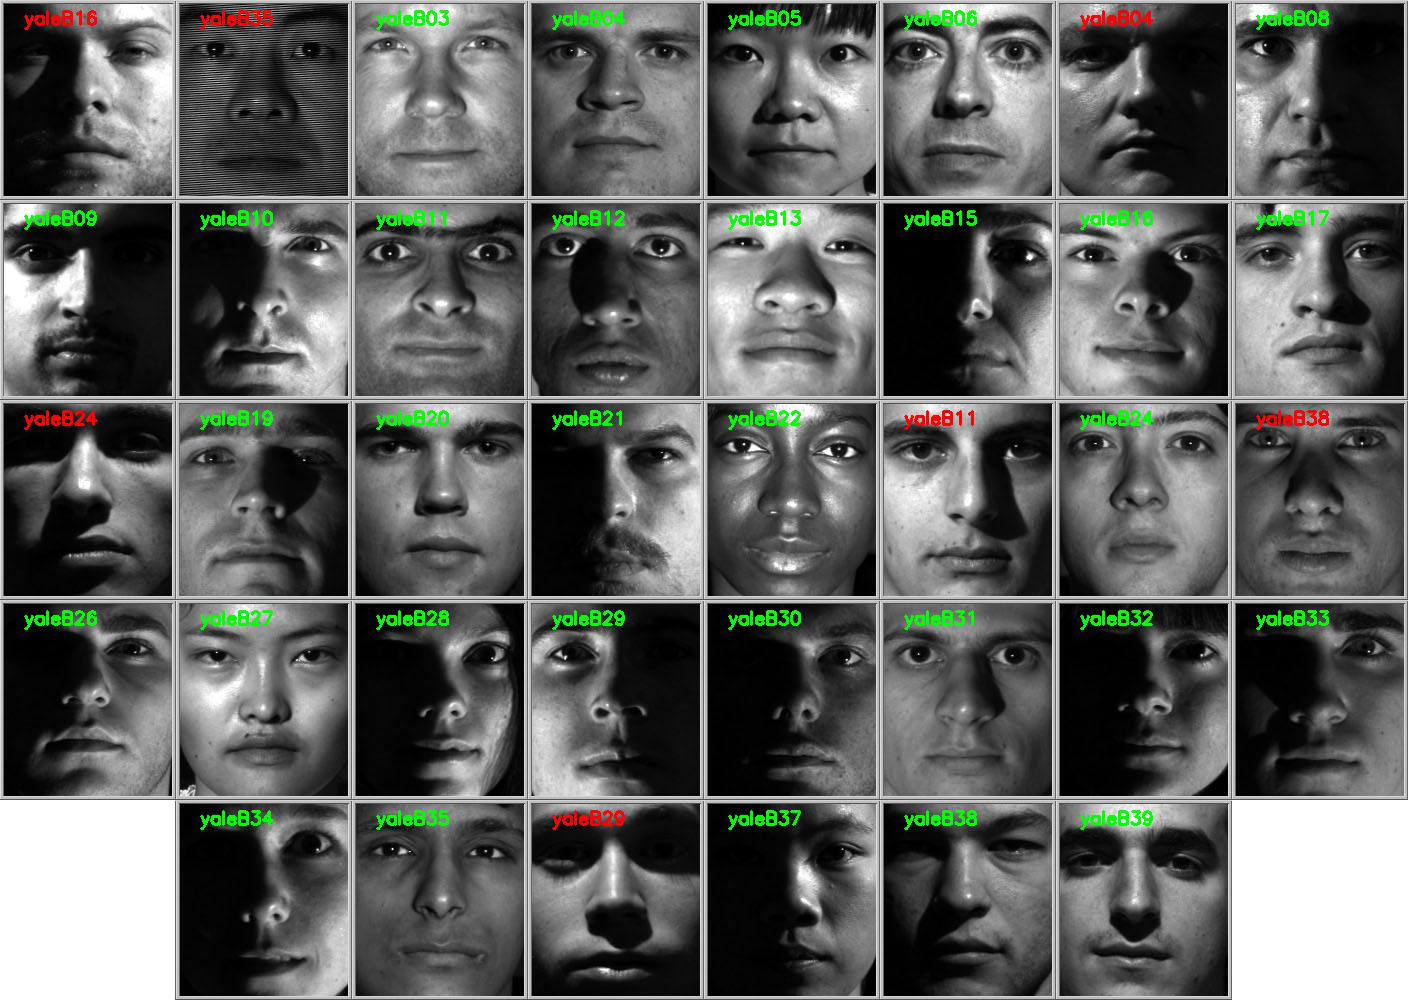
\includegraphics[width=0.95\linewidth]{imagens/eigenfaces_resultado_yale.jpg}
\end{figure}


\Needspace{5\baselineskip}
\subsubsection{Comparação com outros métodos}\label{sec:eigenfaces_comparacao}

Além do Eigenfaces, os métodos Fisherfaces e Local Binary Patterns Histograms também estão implementados na biblioteca OpenCV. Para fins de comparação, os testes realizados com o Eigenfaces também foram realizados com esses dois métodos. Os resultados podem ser vistos na \autoref{tab:compara_reconhecimento} \footnotemark.

\begin{table}[htpb]
\centering
\caption{Bancos de faces utilizados para testes}
\label{tab:bancos_faces}
\begin{tabular}{|l|l|l|}
\hline
\textbf{Banco de faces} & \textbf{Indivíduos} & \textbf{Fotos de treino} \\\hline
\textbf{AT\&T}          & 40                  & 360                      \\\hline
\textbf{FERET}          & 865                 & 1542                     \\\hline
\textbf{Extended Yale}  & 38                  & 1862                     \\\hline
\end{tabular}
\end{table}

\begin{table}[htbp]
\centering
\caption{Comparação dos algoritmos de reconhecimento facial}
\label{tab:compara_reconhecimento}
\begin{tabular}{|c|l|l|l|l|}
\hline
\textbf{Método}                       & \textbf{Banco de faces} & \textbf{Acertos} & \textbf{Erros} & \textbf{Taxa de acertos} \\\hline
\multirow{3}{*}{\textbf{Eigenfaces}}  & AT\&T                   & 38               & 2              & 95,0\%                   \\
                                      & FERET                   & 550              & 315            & 63,4\%                   \\
                                      & Extended Yale           & 31               & 7              & 81,6\%                   \\\hline
\multirow{3}{*}{\textbf{Fisherfaces}} & AT\&T                   & 39               & 1              & 97,5\%                   \\
                                      & FERET\footnotemark[\value{footnote}] & -   & -              & -                        \\
                                      & Extended Yale           & 38               & 0              & 100\%                    \\\hline
\multirow{3}{*}{\textbf{LBPH}}        & AT\&T                   & 40               & 40             & 100\%                    \\
                                      & FERET                   & 786              & 81             & 90,7\%                   \\
                                      & Extended Yale           & 36               & 2              & 94,7\%                   \\\hline
\end{tabular}
\end{table}

\footnotetext{Devido à pouca quantidade de imagens por indivíduo, o teste com a FERET não pode ser realizado com o Fisherfaces.}

Pelos resultados obtidos nos testes realizados neste trabalho e em outros artigos, pode-se concluir que o método de reconhecimento utilizando eigenfaces é bastante rudimentar quando comparado a métodos mais recentes. Seu estudo é importante por ter sido um pioneiro na área de reconhecimento e servido de base para outros algoritmos, porém seu desempenho deixa a desejar, especialmente em ambientes pouco controlados.

% ----------------------------------------------------------
% Capitulo 5
% ----------------------------------------------------------
\chapter{Projeto do sistema}\label{cap:projeto}

O sistema proposto será composto por dois módulos.
O primeiro corresponde à etapa de captura de fotos, detecção facial e upload das faces a serem processadas pelo segundo módulo, que, por sua vez, extrai características como idade, emoções e gênero e tenta verificar se a mesma face já foi analisada no passado.

\section{Módulo 1}\label{sec:modulo1}

O módulo 1 é o foco deste trabalho. Sua principal função é capturar as fotos a serem analisadas no segundo módulo.
Para minimizar o volume de dados trafegados pela rede e concentrar os esforços dos algoritmos de análise apenas nas áreas de interesse, o primeiro módulo não pode enviar todas as imagens capturadas, sendo necessário um pré-processamento que ignore as fotos que não contenham faces e também remova o fundo das fotos que contenham faces.

\subsection{Raspberry Pi}

Câmeras comuns não possuem poder computacional para realizar o pré-processamento desejado e computadores tradicionais são caros, grandes e muito pesados para esse propósito.

O meio termo ideal são os computadores de baixo custo em placa única, que podem ser posicionados de forma discreta e, apesar de limitados, são capazes de executar sistemas operacionais como o Linux ARM.

\begin{figure}[htbp]
    \centering
    \caption{Raspberry Pis com câmera}
    \label{fig:raspberry}
    \begin{subfigure}[t]{0.49\textwidth}
    \centering
    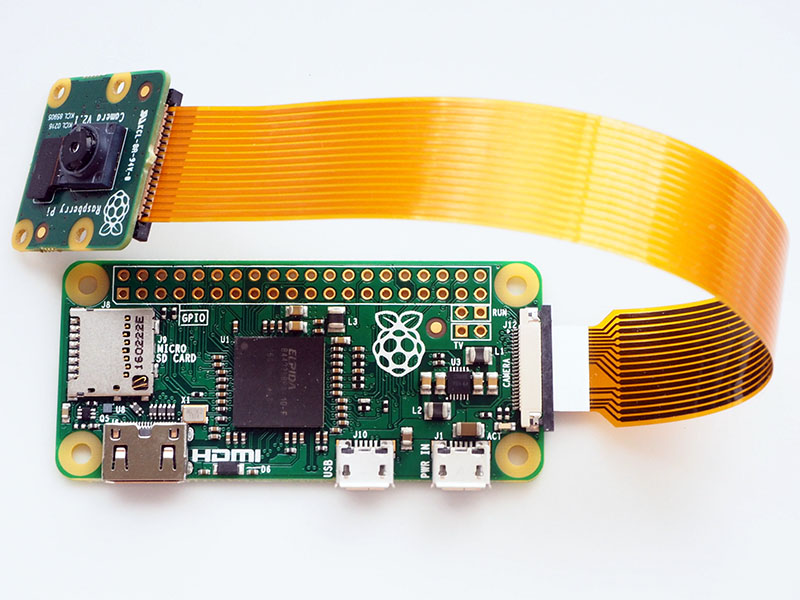
\includegraphics[width=0.95\linewidth]{imagens/raspberry_zero.jpg}
    \caption{Raspberry Pi Zero. Fonte: \cite{upton2016zero}} \label{fig:raspberry:a}
    \end{subfigure}
    \begin{subfigure}[t]{0.49\textwidth}
    \centering
    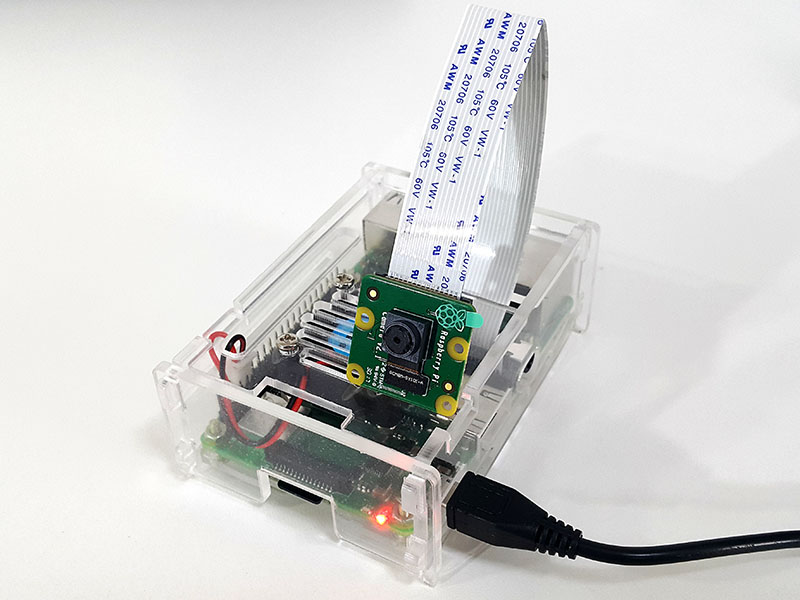
\includegraphics[width=0.95\linewidth]{imagens/raspberry.jpg}
    \caption{Raspberry Pi 3 modelo B+ em um case de acrílico} \label{fig:raspberry:b}
    \end{subfigure}
\end{figure}

O computador escolhido para este projeto foi o Raspberry Pi nos modelos Raspberry Pi Zero (\autoref{fig:raspberry:a}) e Raspberry Pi 3 B+ (\autoref{fig:raspberry:b}) devido ao seu baixo custo, alta disponibilidade e por possuir interface para câmera (CSI). O projeto completo custou menos de R\$ 500,00.

O Raspberry Pi Zero possui um processador ARM single-core de 1 GHz e 512 MB de memória SDRAM, enquanto que o Raspberry Pi 3 modelo B+ possui um processador quad-core 64-bit de 1,4 GHz e 1 GB de memória SDRAM.

O sistema operacional escolhido para ser instalado no Raspberry Pi foi o Raspbian Stretch Lite, uma distribuição de Linux baseada no Debian otimizada especificamente para o Raspberry Pi.

\subsection{Detecção facial}

O programa para selecionar apenas as regiões com faces deve utilizar um algoritmo eficiente de detecção facial capaz de ser executado a pelo menos um quadro por segundo no hardware e sistema operacional escolhidos.

O algoritmo de detecção facial selecionado para o primeiro módulo foi o Viola-Jones, pois, como estudado em capítulos anteriores, ele é eficiente o suficiente para ser executado em tempo real e está implementado na biblioteca multiplataforma OpenCV.

O \autoref{cod:detector_opencv_picamera} apresenta a implementação do sistema de detecção facial utilizando a câmera do Raspberry Pi.

\section{Módulo 2}\label{sec:modulo2}

O segundo módulo \ldots

% Finaliza a parte no bookmark do PDF
% para que se inicie o bookmark na raiz
% e adiciona espaço de parte no Sumário
% ----------------------------------------------------------
\phantompart

% ----------------------------------------------------------
% Conclusão (outro exemplo de capítulo sem numeração e presente no sumário)
% ----------------------------------------------------------
%\chapter*[Conclusão]{Conclusão}
%\addcontentsline{toc}{chapter}{Conclusão}
% ----------------------------------------------------------
\chapter{Conclusão}

Este trabalho mostrou...

As principais contribuições deste trabalho são...


% ----------------------------------------------------------
% ELEMENTOS PÓS-TEXTUAIS
% ----------------------------------------------------------
\postextual
% ----------------------------------------------------------

% ----------------------------------------------------------
% Referências bibliográficas
% ----------------------------------------------------------
\bibliography{elementos-postextuais/referencias}

% ----------------------------------------------------------
% Glossário
% ----------------------------------------------------------
%
% Consulte o manual da classe abntex2 para orientações sobre o glossário.
%
%\glossary

% ----------------------------------------------------------
% Apêndices
% ----------------------------------------------------------
% ----------------------------------------------------------
% Apêndices
% ----------------------------------------------------------

% Inicia os apêndices
\begin{apendicesenv}

% Imprime uma página indicando o início dos apêndices
\partapendices

\chapter{Código do detector facial}\label{cap:anexo_detector_facial_opencv}

\begin{code}
\caption{Detector facial usando a biblioteca OpenCV}
\label{cod:detector_facial_opencv}
\inputminted{python}{codigos/detector_facial.py}
\end{code}
% ----------------------------------------------------------

\chapter{Código para Raspberry Pi do detector facial usando OpenCV}\label{cap:anexo_detector_raspberry}

\begin{code}
\caption{Detector facial usando OpenCV e picamera}
\label{cod:detector_opencv_picamera}
\inputminted{python}{codigos/detector_facial_picamera.py}
\end{code}
% ----------------------------------------------------------

\chapter{Código usado para gerar gráficos para ilustrar funcionamento do PCA}\label{cap:ilustra_pca}

\begin{code}
\caption{Código gerador dos gráficos da \autoref{fig:pca}}
\label{cod:ilustra_pca}
\inputminted{python}{codigos/eigenfaces.py}
\end{code}
% ----------------------------------------------------------

\chapter{Código usado para obter imagens da face média e dos componentes principais}\label{cap:pca_opencv}

\begin{code}
\caption{Ilustração }
\label{cod:pca_opencv}
\inputminted{python}{codigos/eigenfaces.py}
\end{code}
% ----------------------------------------------------------

\chapter{Código do reconhecedor de faces por Eigenfaces usando OpenCV}\label{cap:eigenfaces_opencv}

\begin{code}
\caption{Reconhecimento facial por Eigenfaces usando OpenCV}
\label{cod:eigenfaces_opencv}
\inputminted{python}{codigos/eigenfaces.py}
\end{code}
% ----------------------------------------------------------

\end{apendicesenv}



% ----------------------------------------------------------
% Anexos
% ----------------------------------------------------------
\anexos
% ----------------------------------------------------------
% Anexos
% ----------------------------------------------------------
% Inicia os anexos
\begin{anexosenv}

% Imprime uma página indicando o início dos anexos
\partanexos

\chapter{Código do AdaBoost}\label{cap:anexo_adaboost_python}

\begin{code}
\caption{AdaBoost. Fonte: \cite{datta2015face}}
\label{cod:adaboost}
\inputminted{python}{codigos/adaboost.py}
\end{code}

\end{anexosenv}


%---------------------------------------------------------------------
% INDICE REMISSIVO
%---------------------------------------------------------------------
\phantompart
\printindex
%---------------------------------------------------------------------

\end{document}
